% Maturarbeit game documentation

\documentclass[11pt, oneside, a4paper]{book}

\usepackage[german]{babel}
\usepackage{quoting,xparse}
\usepackage[colorlinks=false]{hyperref}


\NewDocumentCommand{\bywhom}{m}{% the Bourbaki trick
  {\nobreak\hfill\penalty50\hskip1em\null\nobreak
   \hfill\mbox{\normalfont(#1)}%
   \parfillskip=0pt \finalhyphendemerits=0 \par}%
}

\NewDocumentEnvironment{pquotation}{m}
  {\begin{quoting}[
     indentfirst=true,
     leftmargin=\parindent,
     rightmargin=\parindent]\itshape}
  {\bywhom{#1}\end{quoting}}

% File containing the commands and definitions
% that are used throughout this project.

% Set input encoding
\usepackage[utf8]{inputenc}

% For creating coloured text and backgrounds
\usepackage[table,xcdraw]{xcolor}

% For creating compact lists
\usepackage{paralist}

% To get the current date and time
\usepackage{datetime2}

% For including graphics
\usepackage{graphicx}

% For table positioning
\usepackage{float}

% For glossaries
\usepackage[nonumberlist]{glossaries}
\usepackage[automake, toc]{glossaries-extra}

% For table scaling
\usepackage{array}

% For table formatting
\usepackage{makecell}

% Custom commands

\newcommand{\todo}[1]{TODO: {#1}}

% The following command indicates that its content consists of instructions
% Even if it does not do anything, it is still a good idea to keep instructions within the `instruction` tag to separate them from the rest of the text. One could then typeset them differently, or choose to remove them form the document by redefining the command definition 
\newcommand{\instructions}[1]{#1}

% Uncomment the following command to remove all instructions
% \newcommand{\instructions}[1]{}

% Uncomment the following to make instructions appear in coloured boxes
% Note: The changes within `\instruction` are not visible in latexdiff when they are typeset in this way
% \usepackage{tcolorbox}
% \newcommand{\instructions}[1]{
%     \begin{tcolorbox}[sharp corners, colback=green!30, colframe=green!80!blue, title=Instructions]
%         #1
%     \end{tcolorbox}
% }

% Uncomment the following to make instructions appear in colour.
% Note: The changes within `\instructions` are not visible in latexdiff when they are typeset in this way
% \newcommand{\instructions}[1]{ { \color{blue} #1 } }

% Get a git version description roughly using the idea in  
% https://blog.wxm.be/2013/08/20/automated-git-commit-number-in-latex.html
% Note that the file that is included needs to be generated before the document is built.
% Refer to the makefile for further details.
\IfFileExists{../gitDescription.tmp}
{\newcommand{\gitDescription}{\input{../gitDescription.tmp}}}
{\newcommand{\gitDescription}{Not available}}

% Note: Importing hyperref must be done towards the end since it
% redefines many macros
%
% Note:
%  The following packages must be imported *before* hyperref:
%  
%  The following packages must be imported *after* hyperref:
%    amsrefs, geometry
\usepackage{hyperref}

\usepackage{geometry}



% options for package geometry (influences writable area on page)
% \geometry{a4paper, top=2cm, bottom=2cm}


\makeglossaries

\newglossaryentry{feature}
{
  name={Feature},
  description={Eine bestimmte Funktion, welche die Software weiterbringt}
}

\newglossaryentry{online}
{
  name={Online},
  description={nicht nur lokal auf dem eigenen Rechner sondern im Internet}
}

\newglossaryentry{lokal}
{
  name={Lokal},
  description={Im selben Netz oder Computer}
}

\newglossaryentry{anti-Cheat}
{
  name={Anti-Cheat},
  description={Software um Schummeln zu verhindern.
  Ist sehr komplex und bei allen grösseren online Videospielen vorhanden.
  Teilweise sehr tief in das System vernetzt}
}

\newglossaryentry{cheater}
{
  name={cheater},
  description={Jemand der unerlaubte Methoden oder Programme verwendet, um sich einen unfairen Vorteil zu verschaffen.
  Auf Deutsch \textit{ein Schummler}}
}

\newglossaryentry{Skins}
{
  name={Skins},
  description={Erkaufbare Darstellungen, welche von dem Standard abweichen.
  In vielen Spielen nur im tausch mit echter Währung zu erhalten und bringen nur ästetische Unterschiede}
}

\newglossaryentry{ingame}
{
  name={Ingame},
  description={Im laufendem Spiel, nicht auf dem Computer oder beim Start oder Schliessen des Spiels}
}

\newglossaryentry{pay-to-win}
{
  name={Pay-to-Win},
  description={Übersetzt: Bezahlen-zum-Gewinnen, bedeutet, dass mit echter Währung Ingame Vorteile erkauft werden können}
}

\newglossaryentry{firewall}
{
  name={Firewall},
  description={Schutzsystem eines technischen Systems um Viren fernzuhalten.
  Blockiert aus Sicherheit manchmal mehr als nötig und erschwert so zum Beispiel das verbinden von zwei Computern über das Internet}
}

\newglossaryentry{shop}
{
  name={Shop},
  description={ein Ort im Spiel, in dem Dinge gekauft werden können. Ein Ingame-Laden}
}


\newglossaryentry{multiplayer}
{
  name={Multiplayer},
  description={Mehrspieler, also mehrere Spieler spielen zusammen das gleiche spiel.}
}

\newglossaryentry{singleplayer}
{
  name={Singleplayer},
  description={Einzelspieler, das Spiel wird alleine, meist nur lokal, gepillt}
}

\newglossaryentry{tutorial}
{
  name={Tutorial},
  description={Eine Anleitung, in Videospielen meist eine kurze Spielsequenz, welche Tipps und eine fixe Abfolge besitzt}
}

\newglossaryentry{helden}
{
  name={Helden},
  description={In Videospielen der wichtigste Charakter.
  In gewissen Spielen ist der Held der Charakter den man spielt.
  Der Tod des Heldes bedeutet einen massiven Nachteil}
}

\newglossaryentry{kamera}
{
  name={Kamera},
  description={Die Kamera nimmt in Unity auf, was der Spieler sieht.
  Mit Kamera ist also das gemeint, was der Spieler sieht.}
}

\newglossaryentry{lane}
{
  name={Lane},
  description={
    Bezeichnet generell eine Linie oder Bahn auf der gegangen werden kann.
    Sehr prägnant in MOBAs wie League of Legends oder Dota.
    In unserem Spiel eine Bahn der vier, auf welcher Truppen beschwört werden können.}
}

\newglossaryentry{steam}
{
  name={Steam},
  description={
    Steam ist der grösste Videospiel-Anbieter der Welt.
    Gehört dem Unternehmen Valve.}
}



% \newglossaryentry{slalom}{
%     name={Slalom},
%     description={A kind of \gls{contract} in the \gls{coiffeur-jass} which plays without a trump.
%     Alternates between \gls{bottoms-up} and \gls{tops-down} or vice-versa, scoring rules apply from the first chosen option}
% }


\hypersetup{
    pdfauthor={Marc Honegger, Elia Schürpf},
    pdftitle={Maturarbeit Game Documentation},
}

\begin{document}

\pagestyle{empty}

\frontmatter

\begin{titlepage}

    \begin{center}

        \vspace{1 cm}

        {\Large Maturitätsarbeit 2023 \\ Documentation} \\

        \vspace{1 cm}

        \vspace{0.5cm}

        {\Huge Laneclash}

        \vspace{0.5cm}

        \vspace{1 cm}

        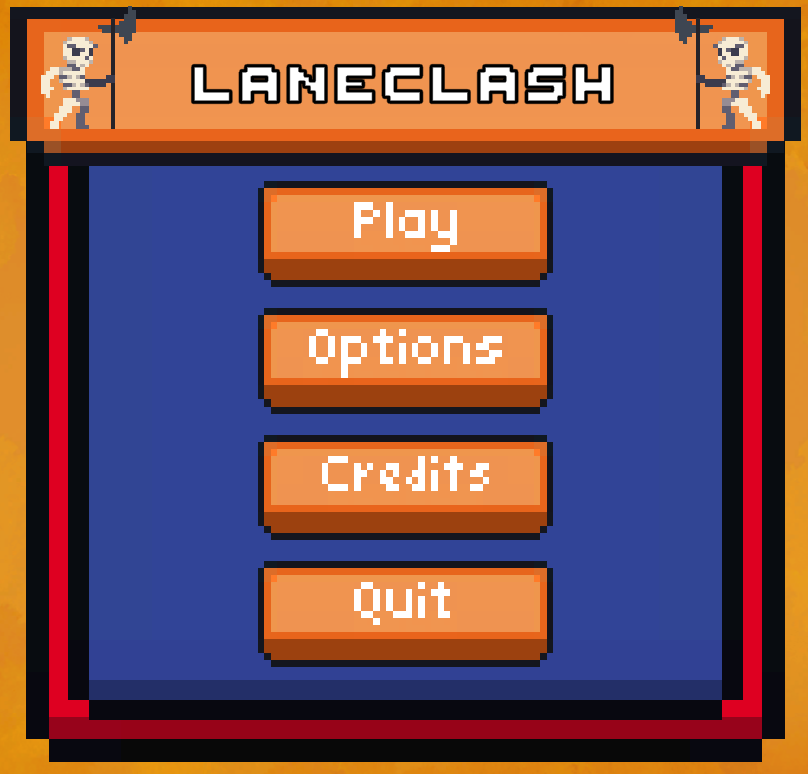
\includegraphics[height=7cm]{resources/laneclash.png}

        \vspace{1 cm}

        Version: 1.0 \\
        Date: \DTMnow \\
        \vspace{1 cm}

        \begin{tabular}{rl}
            \textbf{Team:}          & Marc Honegger (C6a) \\
                                    & Elia Schürpf (C6a)\\
                                    \\
            \textbf{Begleitperson:} & Martin Hunziker
        \end{tabular}

        \vfill

        \vspace{1cm}
        Gymnasium \\
        KZO - Kantonsschule Zürcher Oberland

    \end{center}

\end{titlepage}

\tableofcontents

\mainmatter

\part{Ziel}
\chapter{Vision}

Ein funktionsfähiges Videospiel, welches jede vergleichbare Maturitätsarbeit in den Schatten stellt.
Die Ideen sind nicht neu, sondern waren schon vor Jahren in Marcs Kopf.
Jedoch war für die Umsetzung ein Team notwendig.
Uns war dennoch von Anfang an bewusst,
dass wir auch zu zweit nicht alle Funktionen hinkriegen werden, dennoch haben wir uns ein hohes Ziel gesetzt und für die Betreuung uns für Martin Hunziker entschieden.
Vieles konnten wir schlussendlich auch umsetzen.
Das grösste Wagnis war der Multiplayer und das haben wir dann auch an eigenem Leib erfahren.
Alleine für den Multiplayer wurden über 100h investiert.
Alles in allem kam ein funktionsfähiges und lustiges Spiel heraus.
Einige Kommentare:
\begin{center}
    'Sick Game' - Marc Honegger \\
    'Absolut Krass' - Elia Schürpf \\ 
    'Masterpiece' - Martin Hunziker
\end{center}
Wie das Spiel jetzt aussieht, wie es zu diesem Punkt kommen konnte, aber auch wie es in Zukunft damit weiter geht, ist in dieser Arbeit beschrieben.
\chapter{Ideen}

\renewcommand{\figurename}{Abb.}

\section{Skizzen}

    \begin{figure}[H]
        \centering
        \begin{minipage}[H]{7cm}
        \centering
        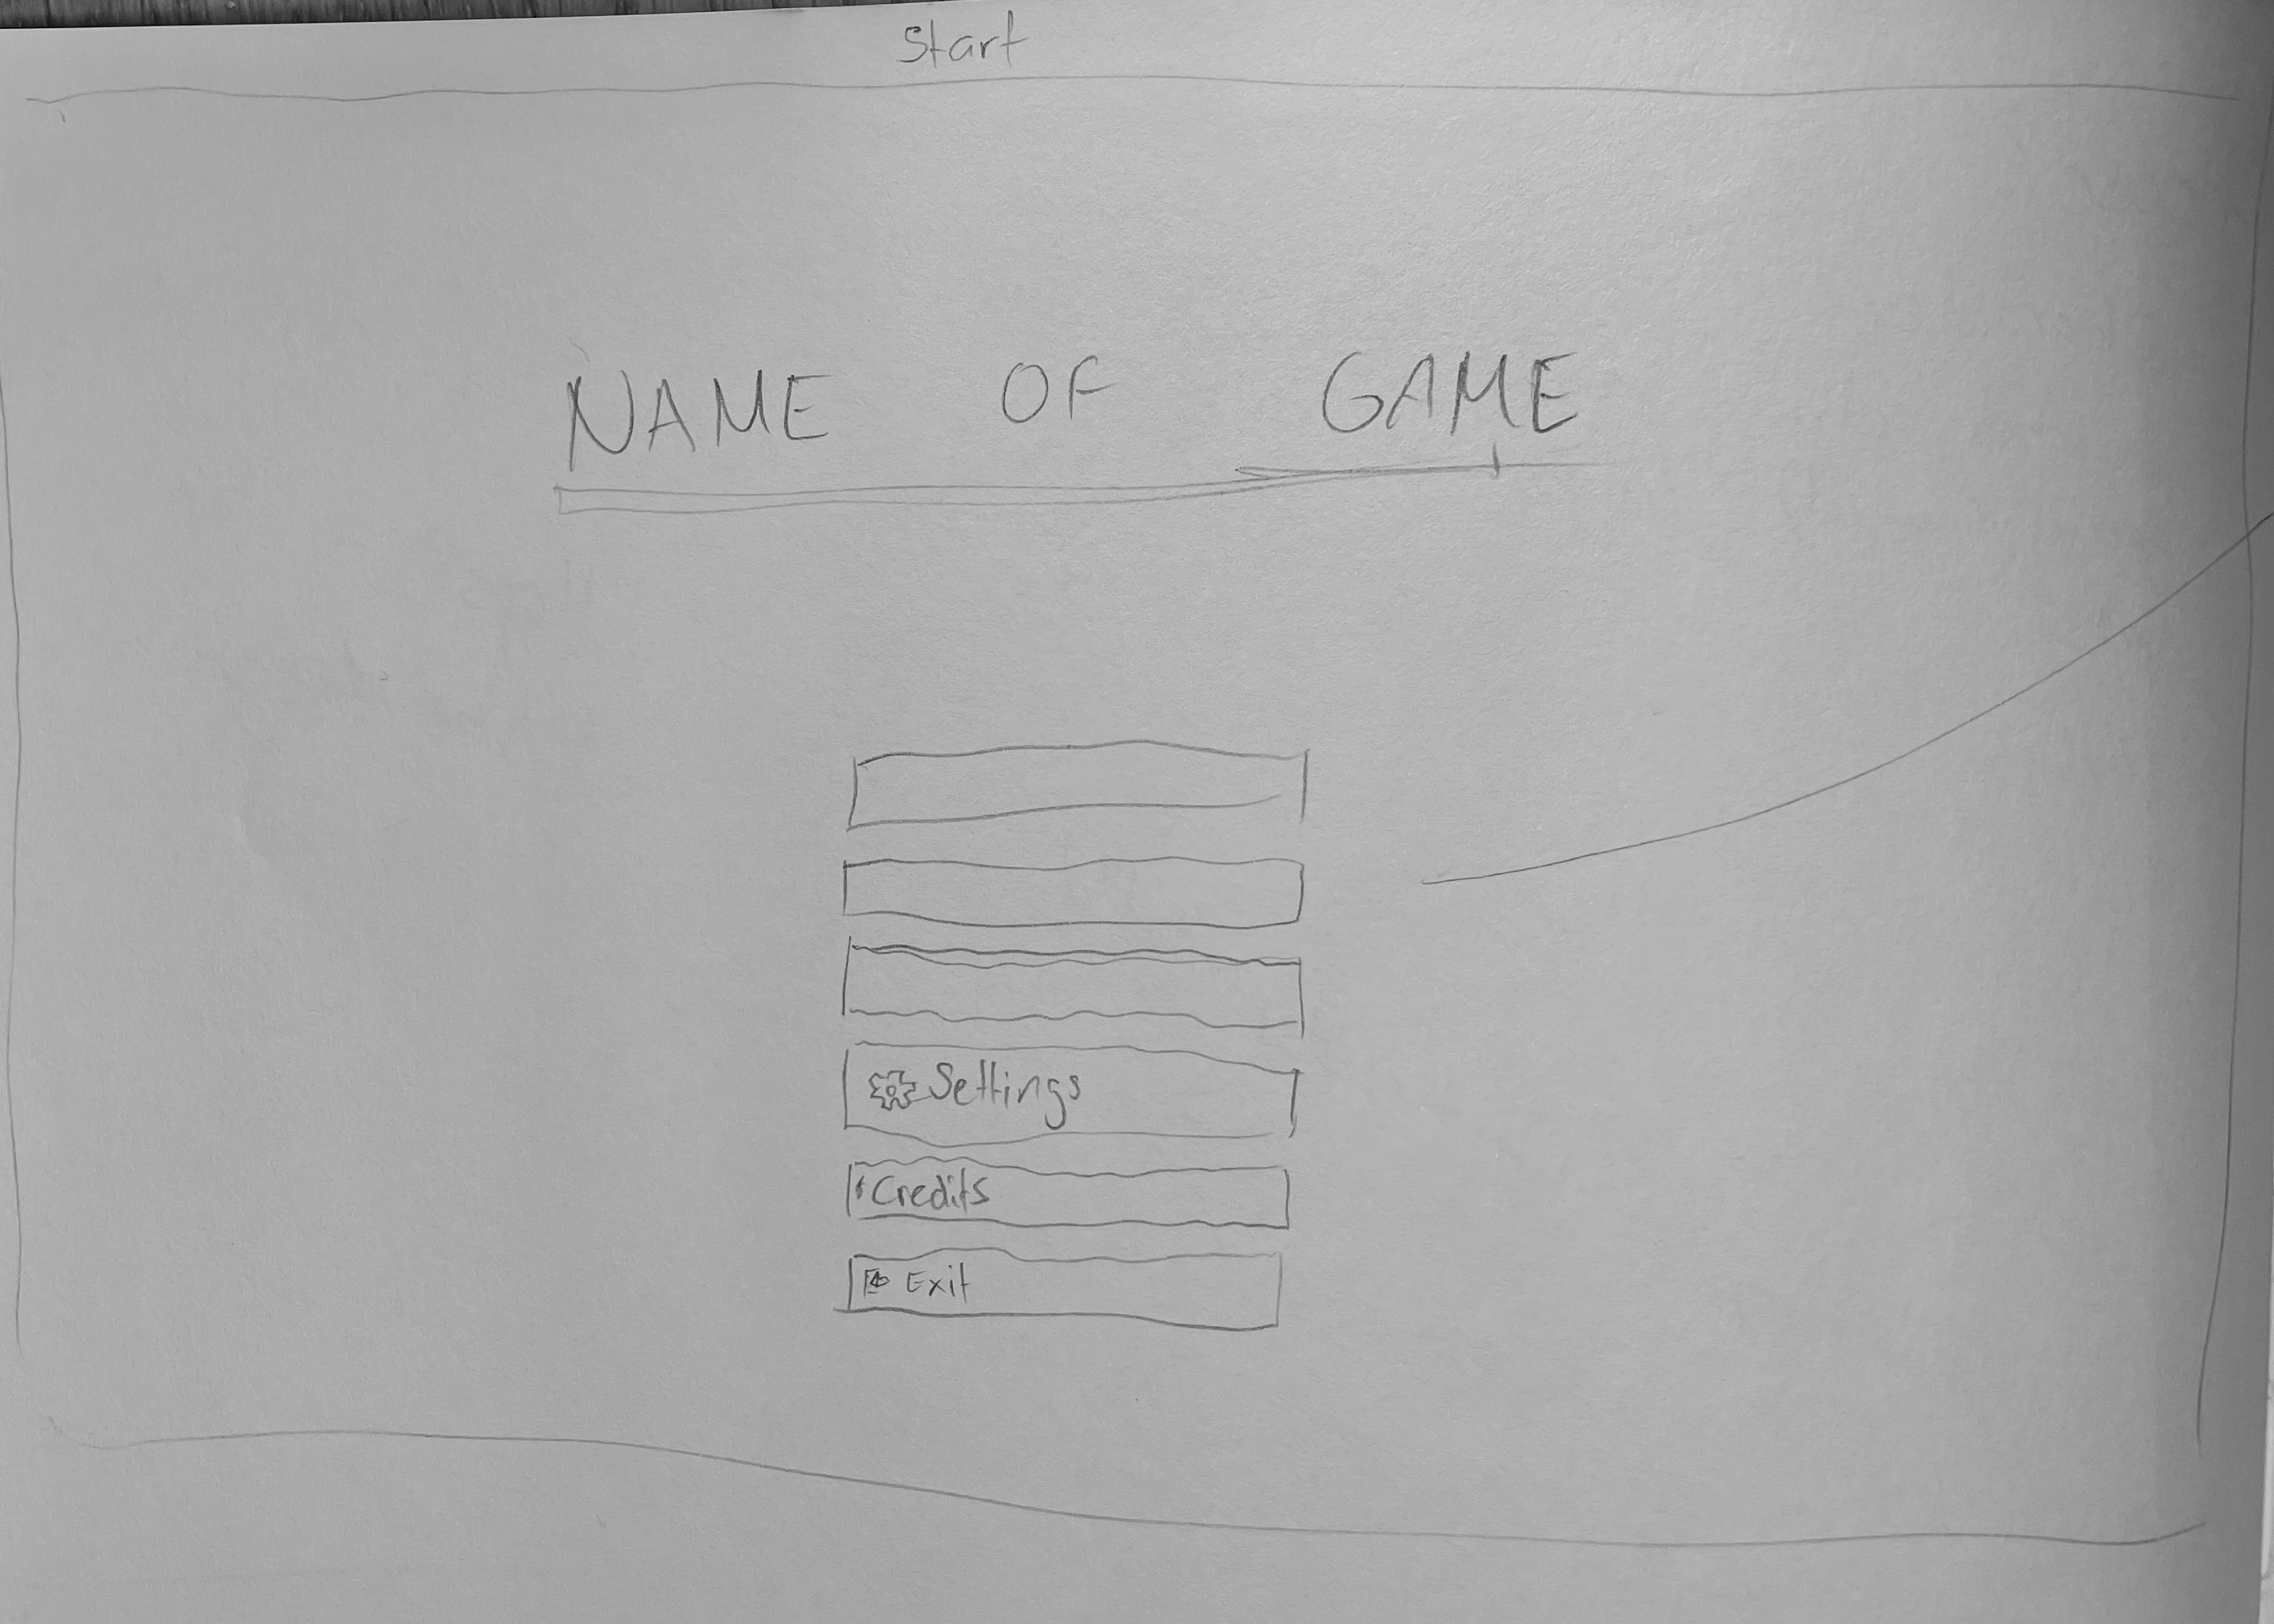
\includegraphics[width=7cm]{resources/Sk_startpage.jpeg}\\
        \caption{Aufbau der Startseite}
        \end{minipage}\hfill
        \begin{minipage}[H]{7cm}
        \centering
        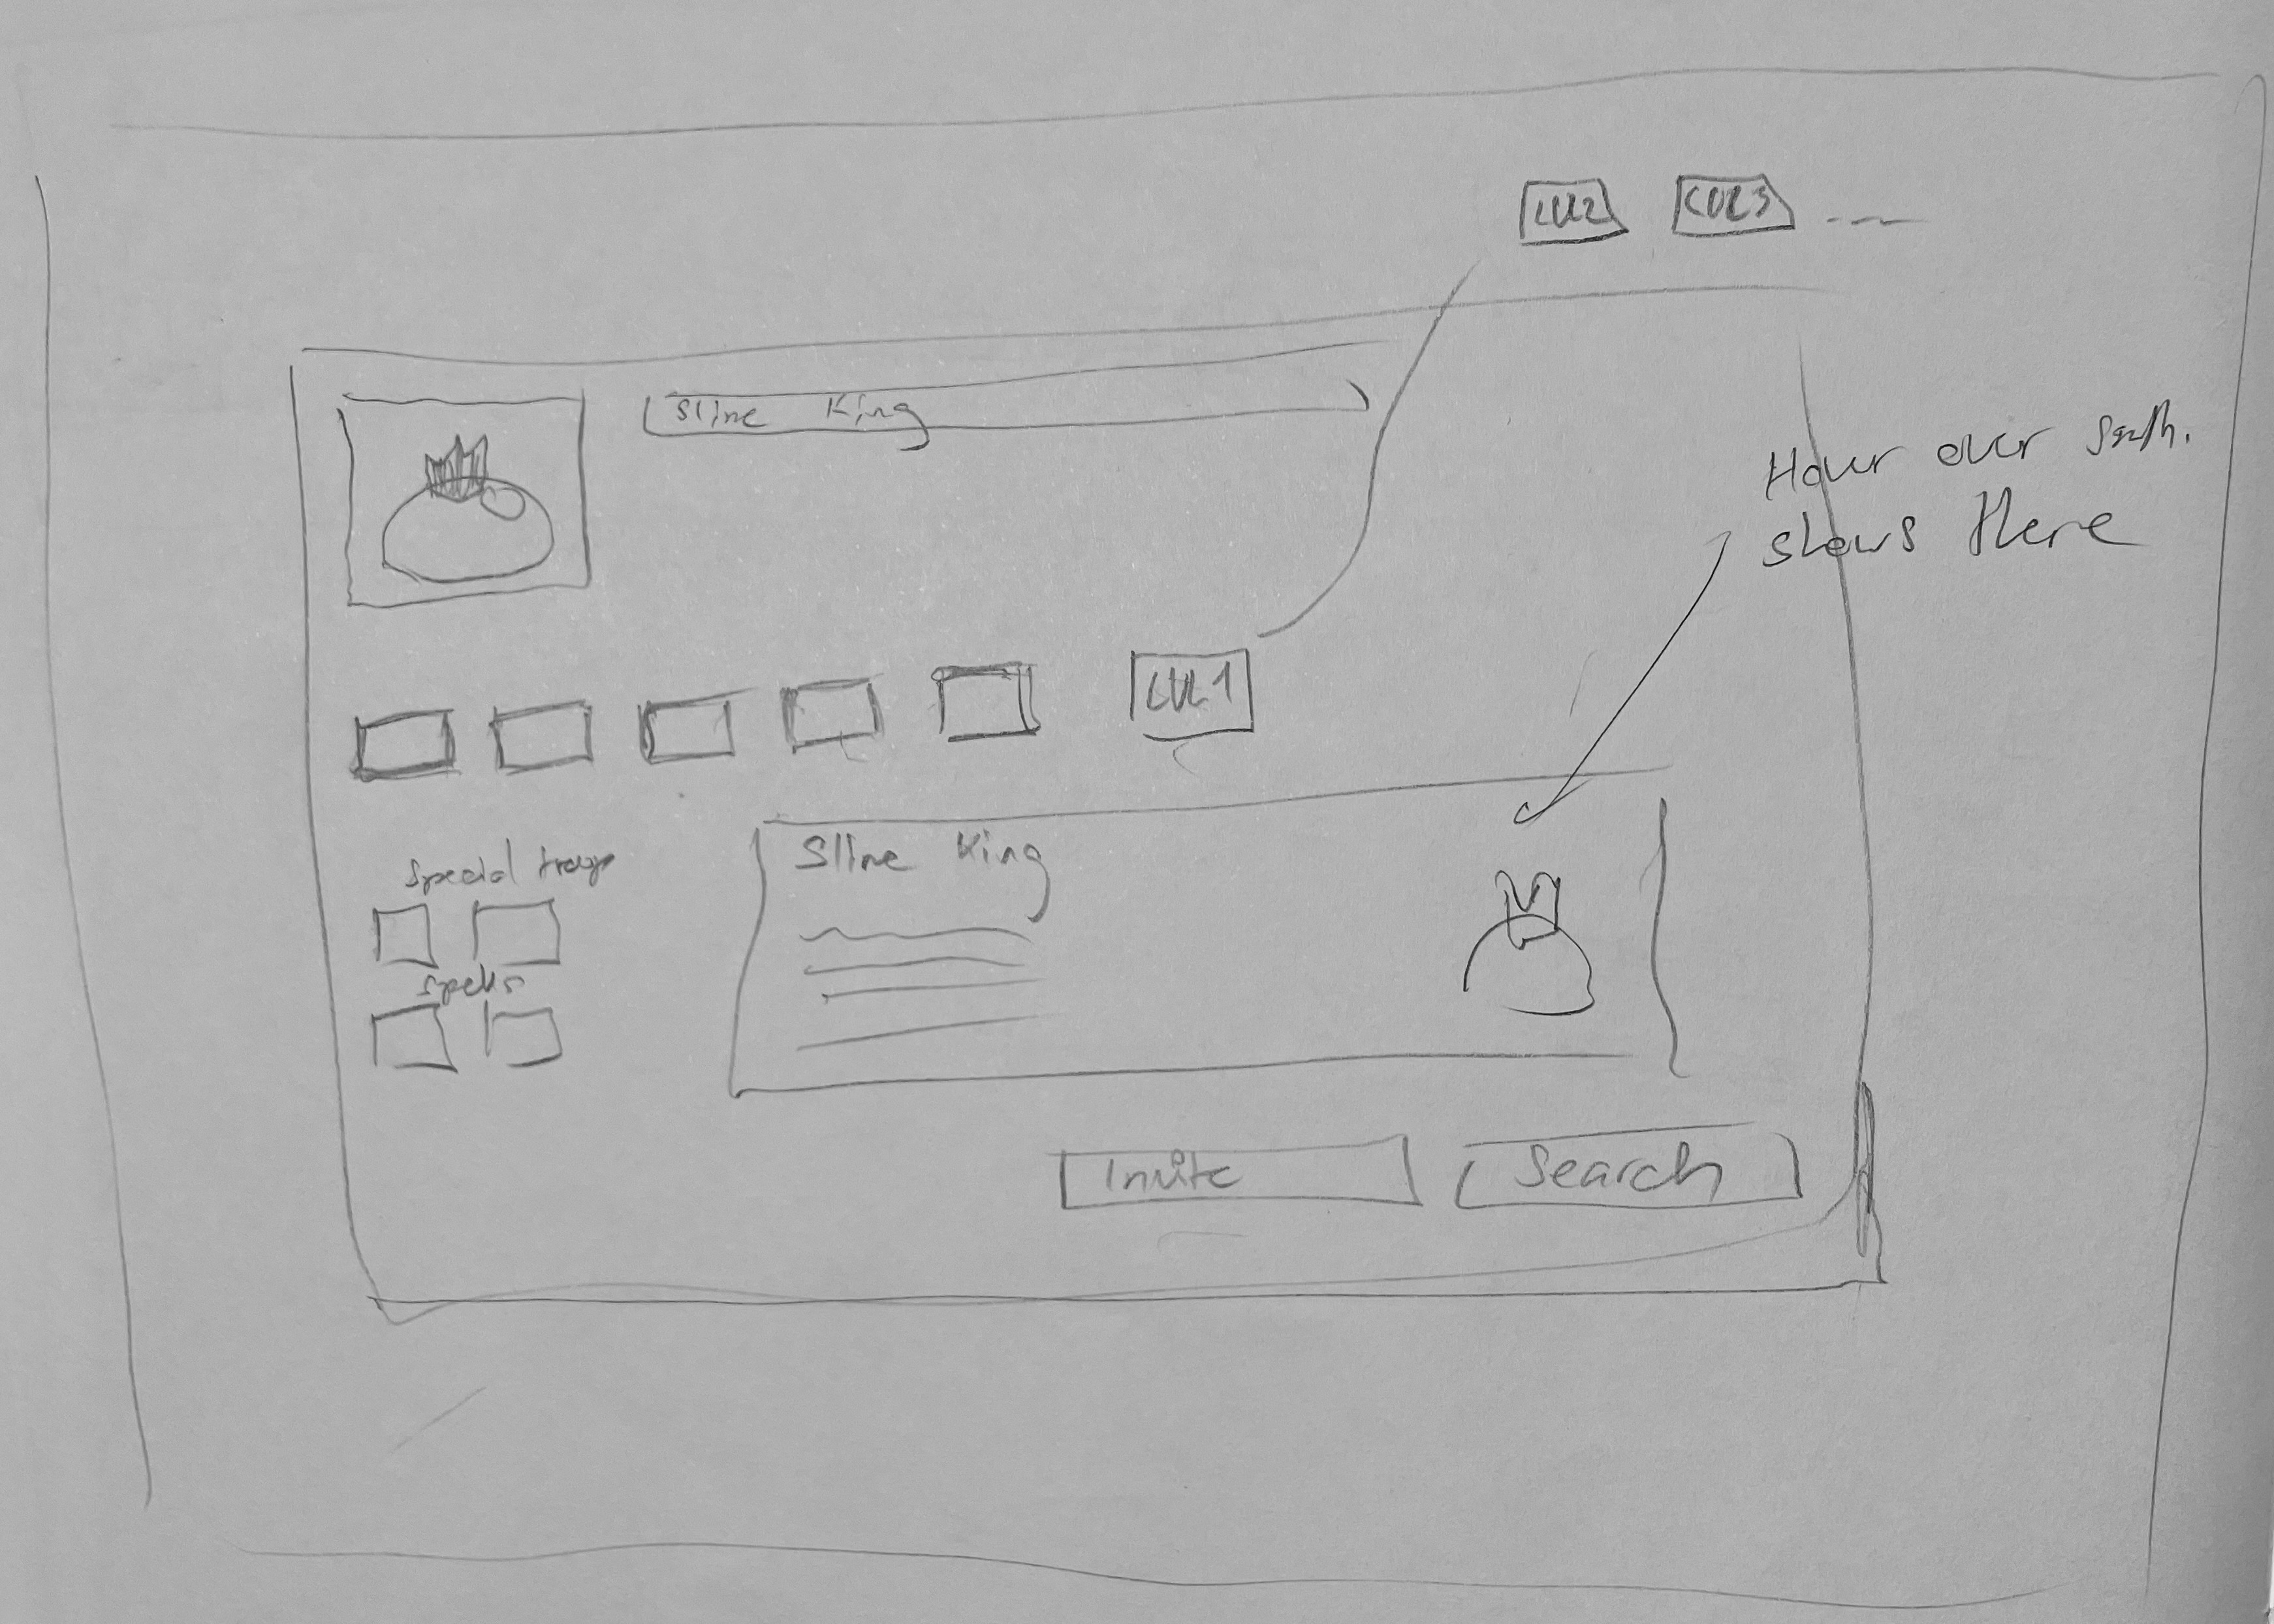
\includegraphics[width=7cm]{resources/SK_auswahl.jpeg}\\
        \caption{Aufbau bei der Deckerstellung}
        \end{minipage}
    \end{figure}
    %\begin{figure}
    %    \centering
    %    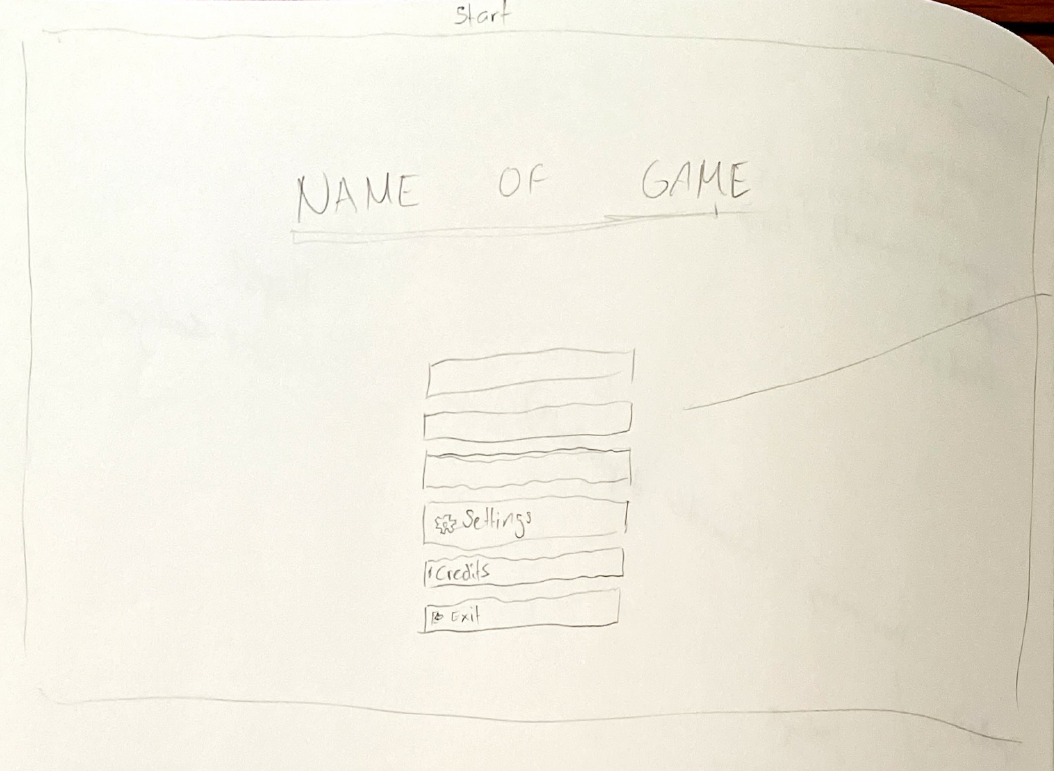
\includegraphics[width=7cm]{resources/SK_startpage.jpeg} \quad 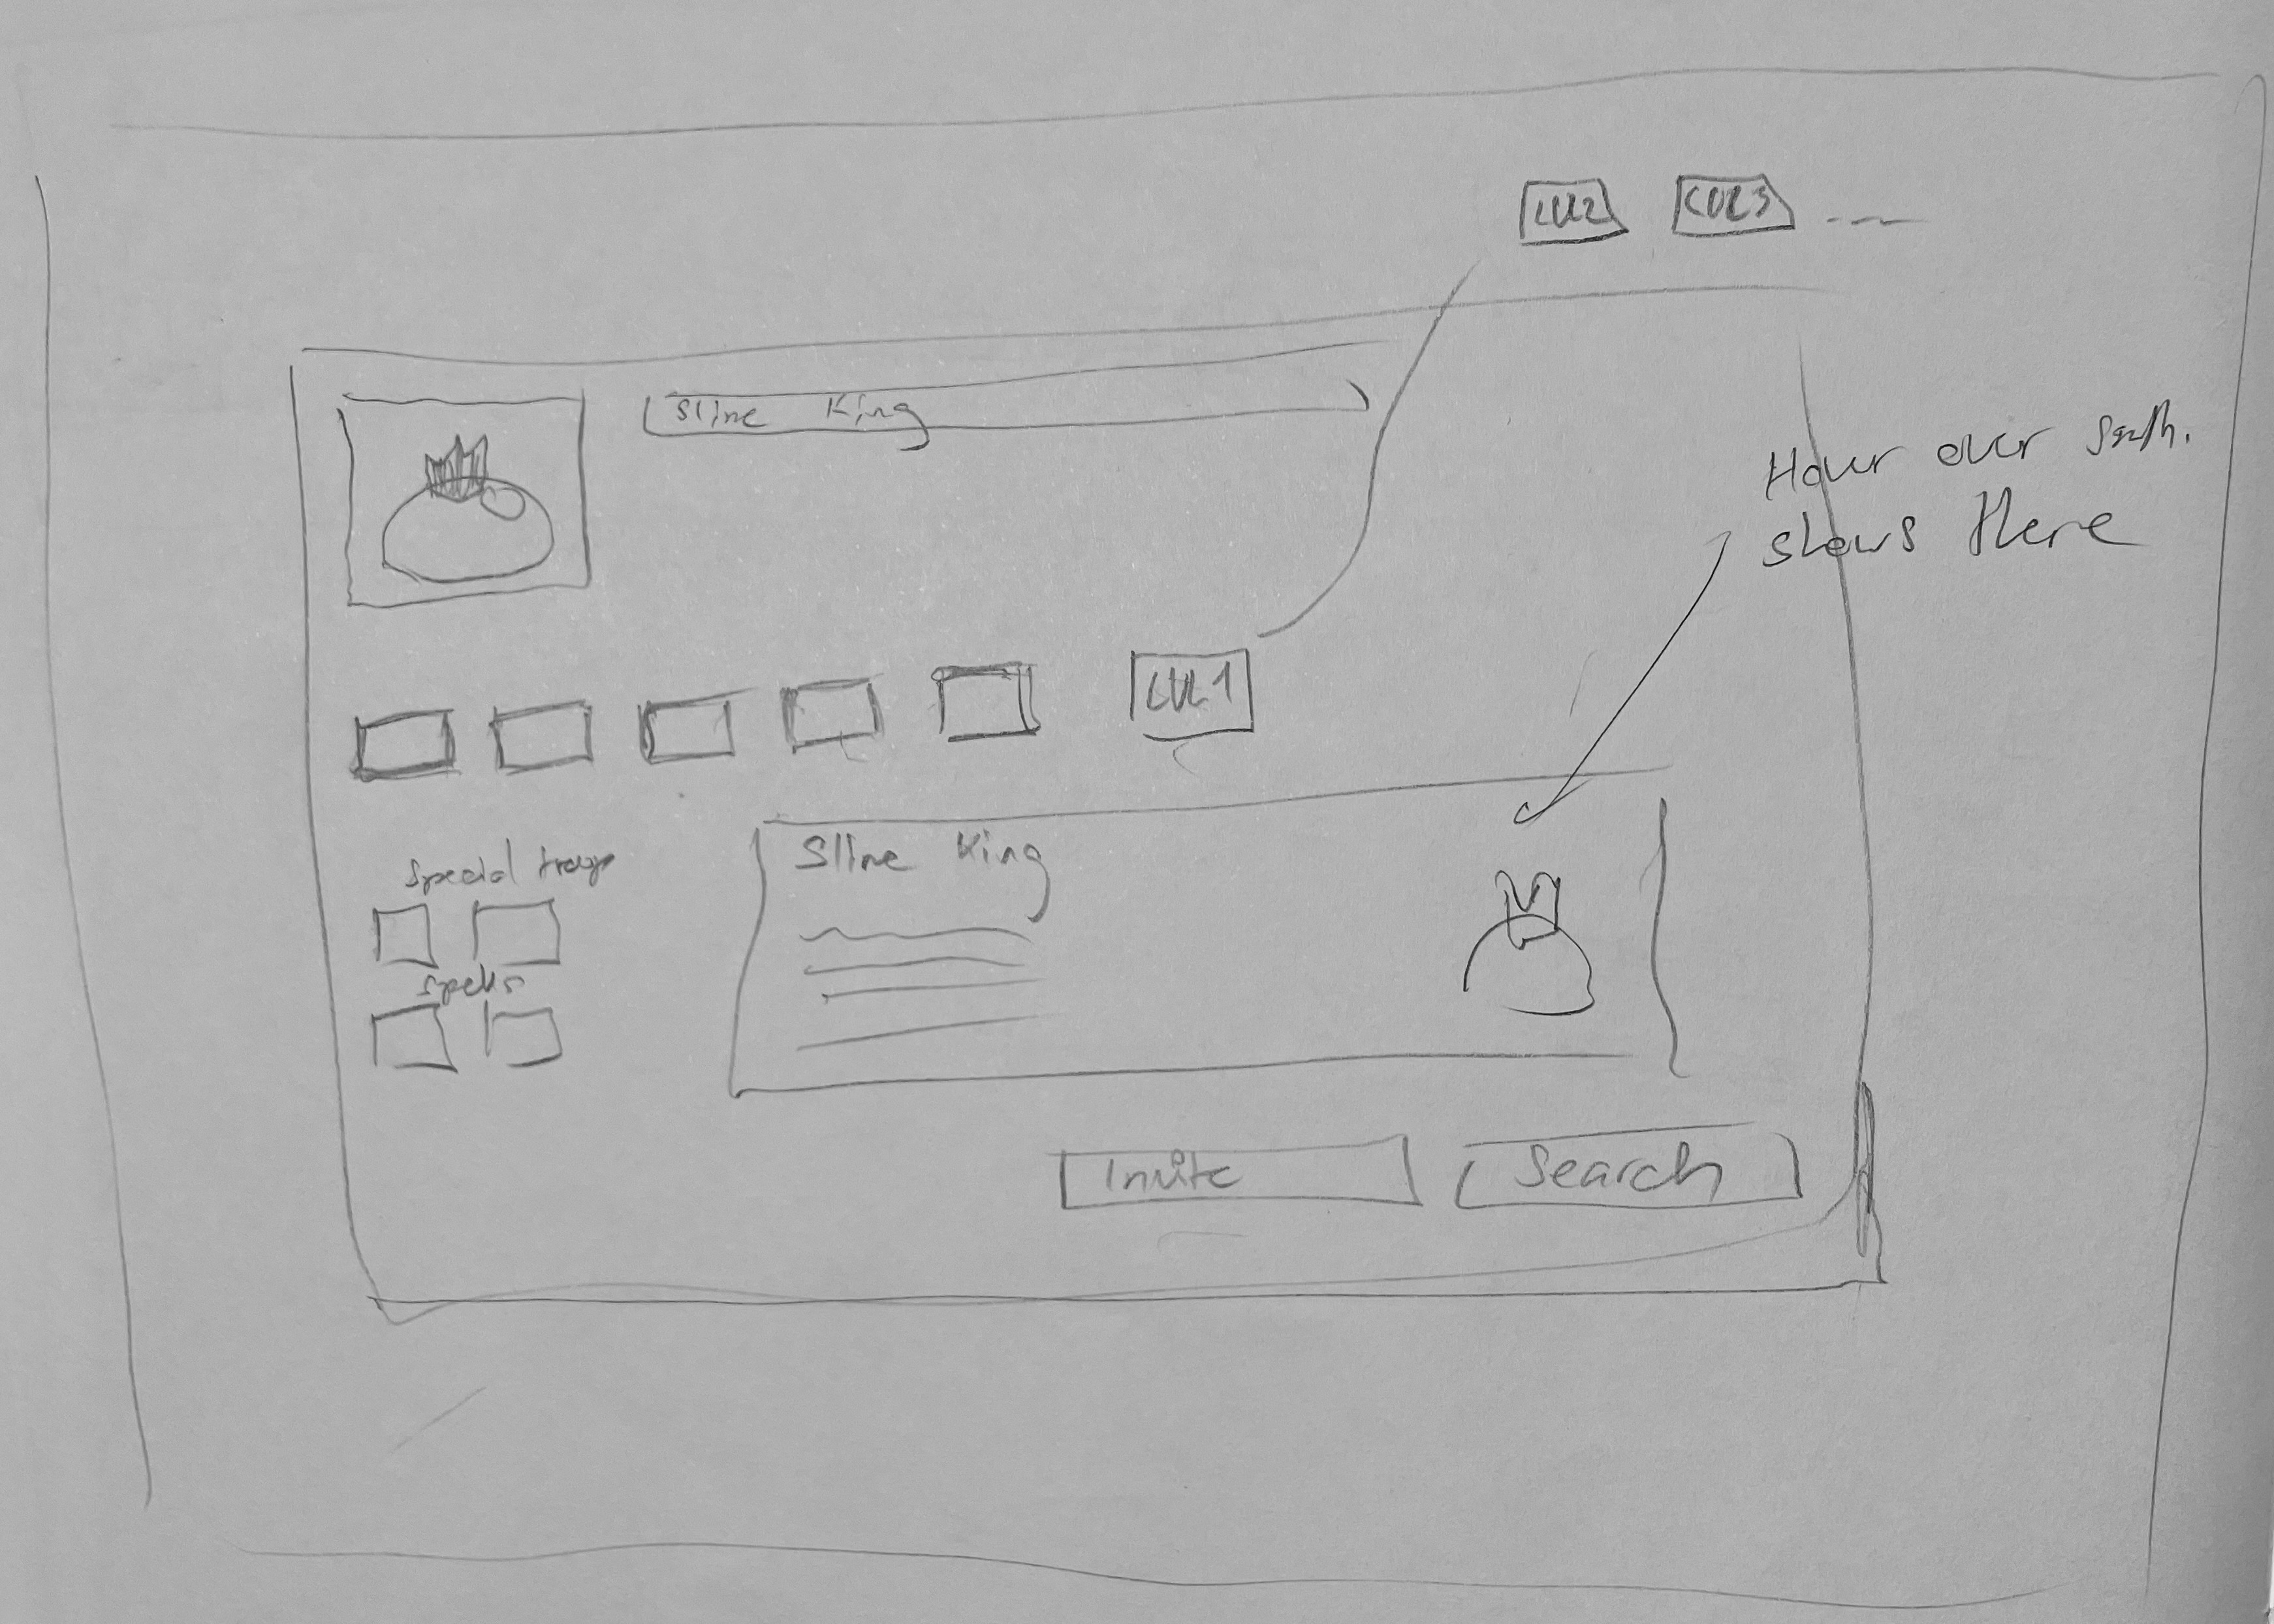
\includegraphics[width=7cm]{resources/SK_auswahl.jpeg}
    %    \caption{hello world} \caption{hello world}
    %\end{figure}
    %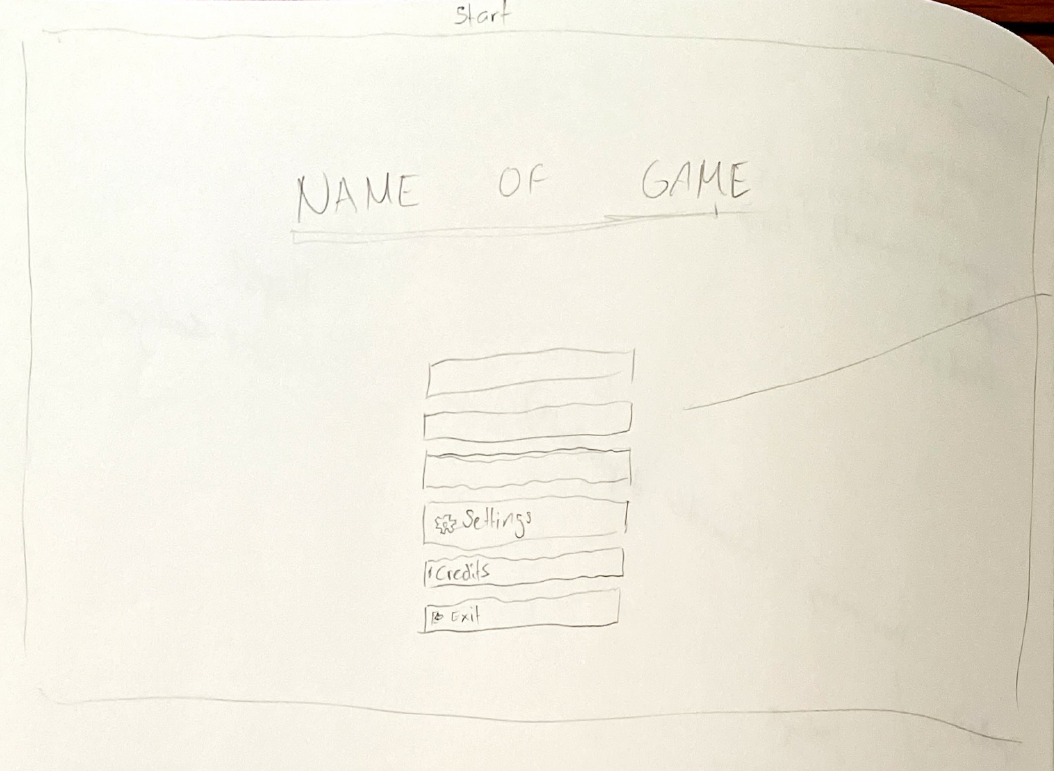
\includegraphics[width=7cm]{resources/SK_startpage.jpeg} \quad 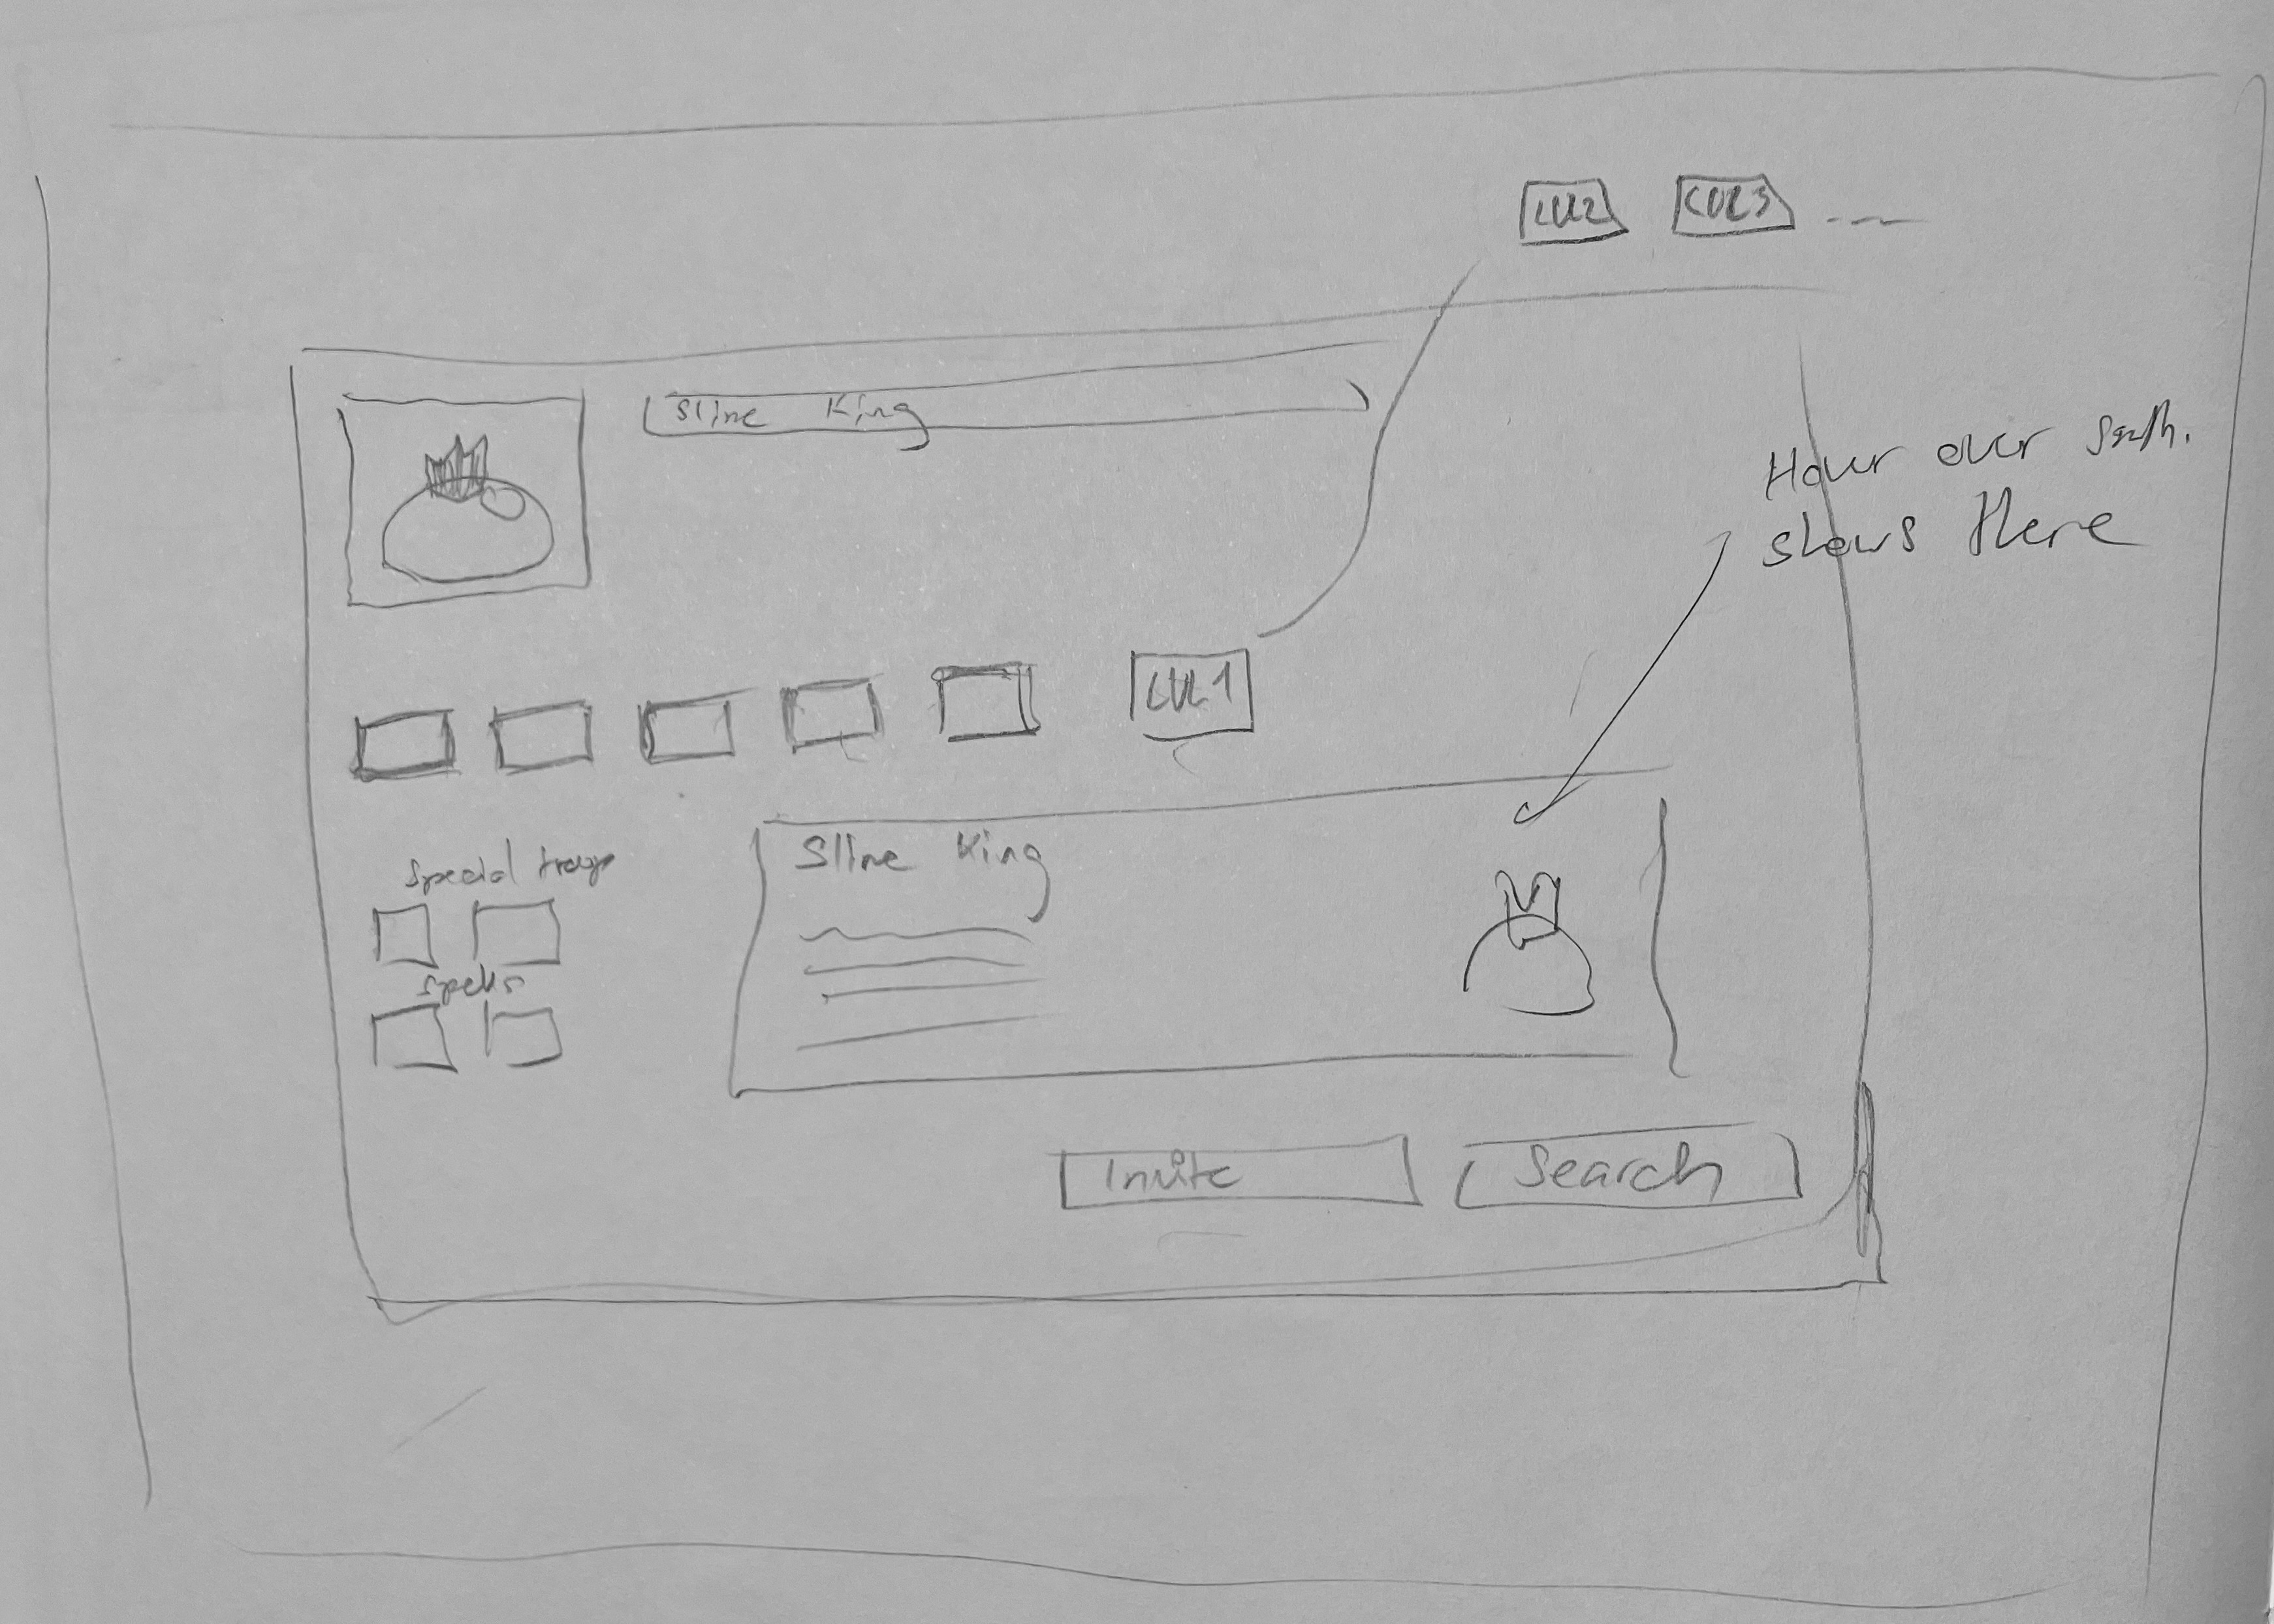
\includegraphics[width=7cm]{resources/SK_auswahl.jpeg}\\
    %\textit{Startseite} \qquad \qquad \qquad \qquad \qquad \qquad \qquad \quad \textit{Auswählen von Karten und Helden}
    \begin{figure}[H]
        \centering
        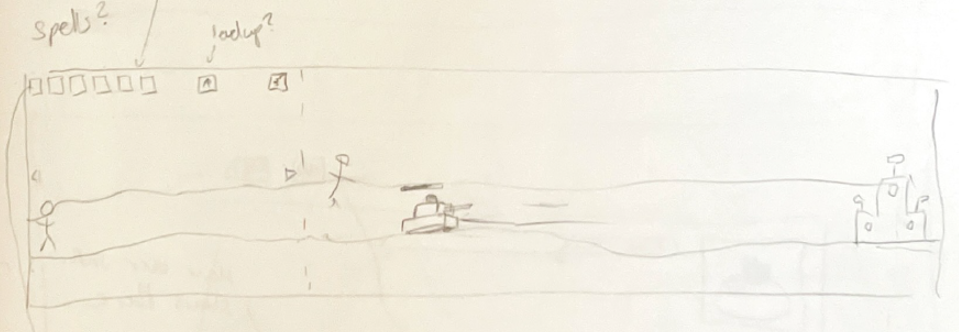
\includegraphics[width=14.5cm]{resources/sk_gamemain.jpeg}\\
        \caption{Spieleszene mit UI}
    \end{figure}

    \begin{figure}[H]
        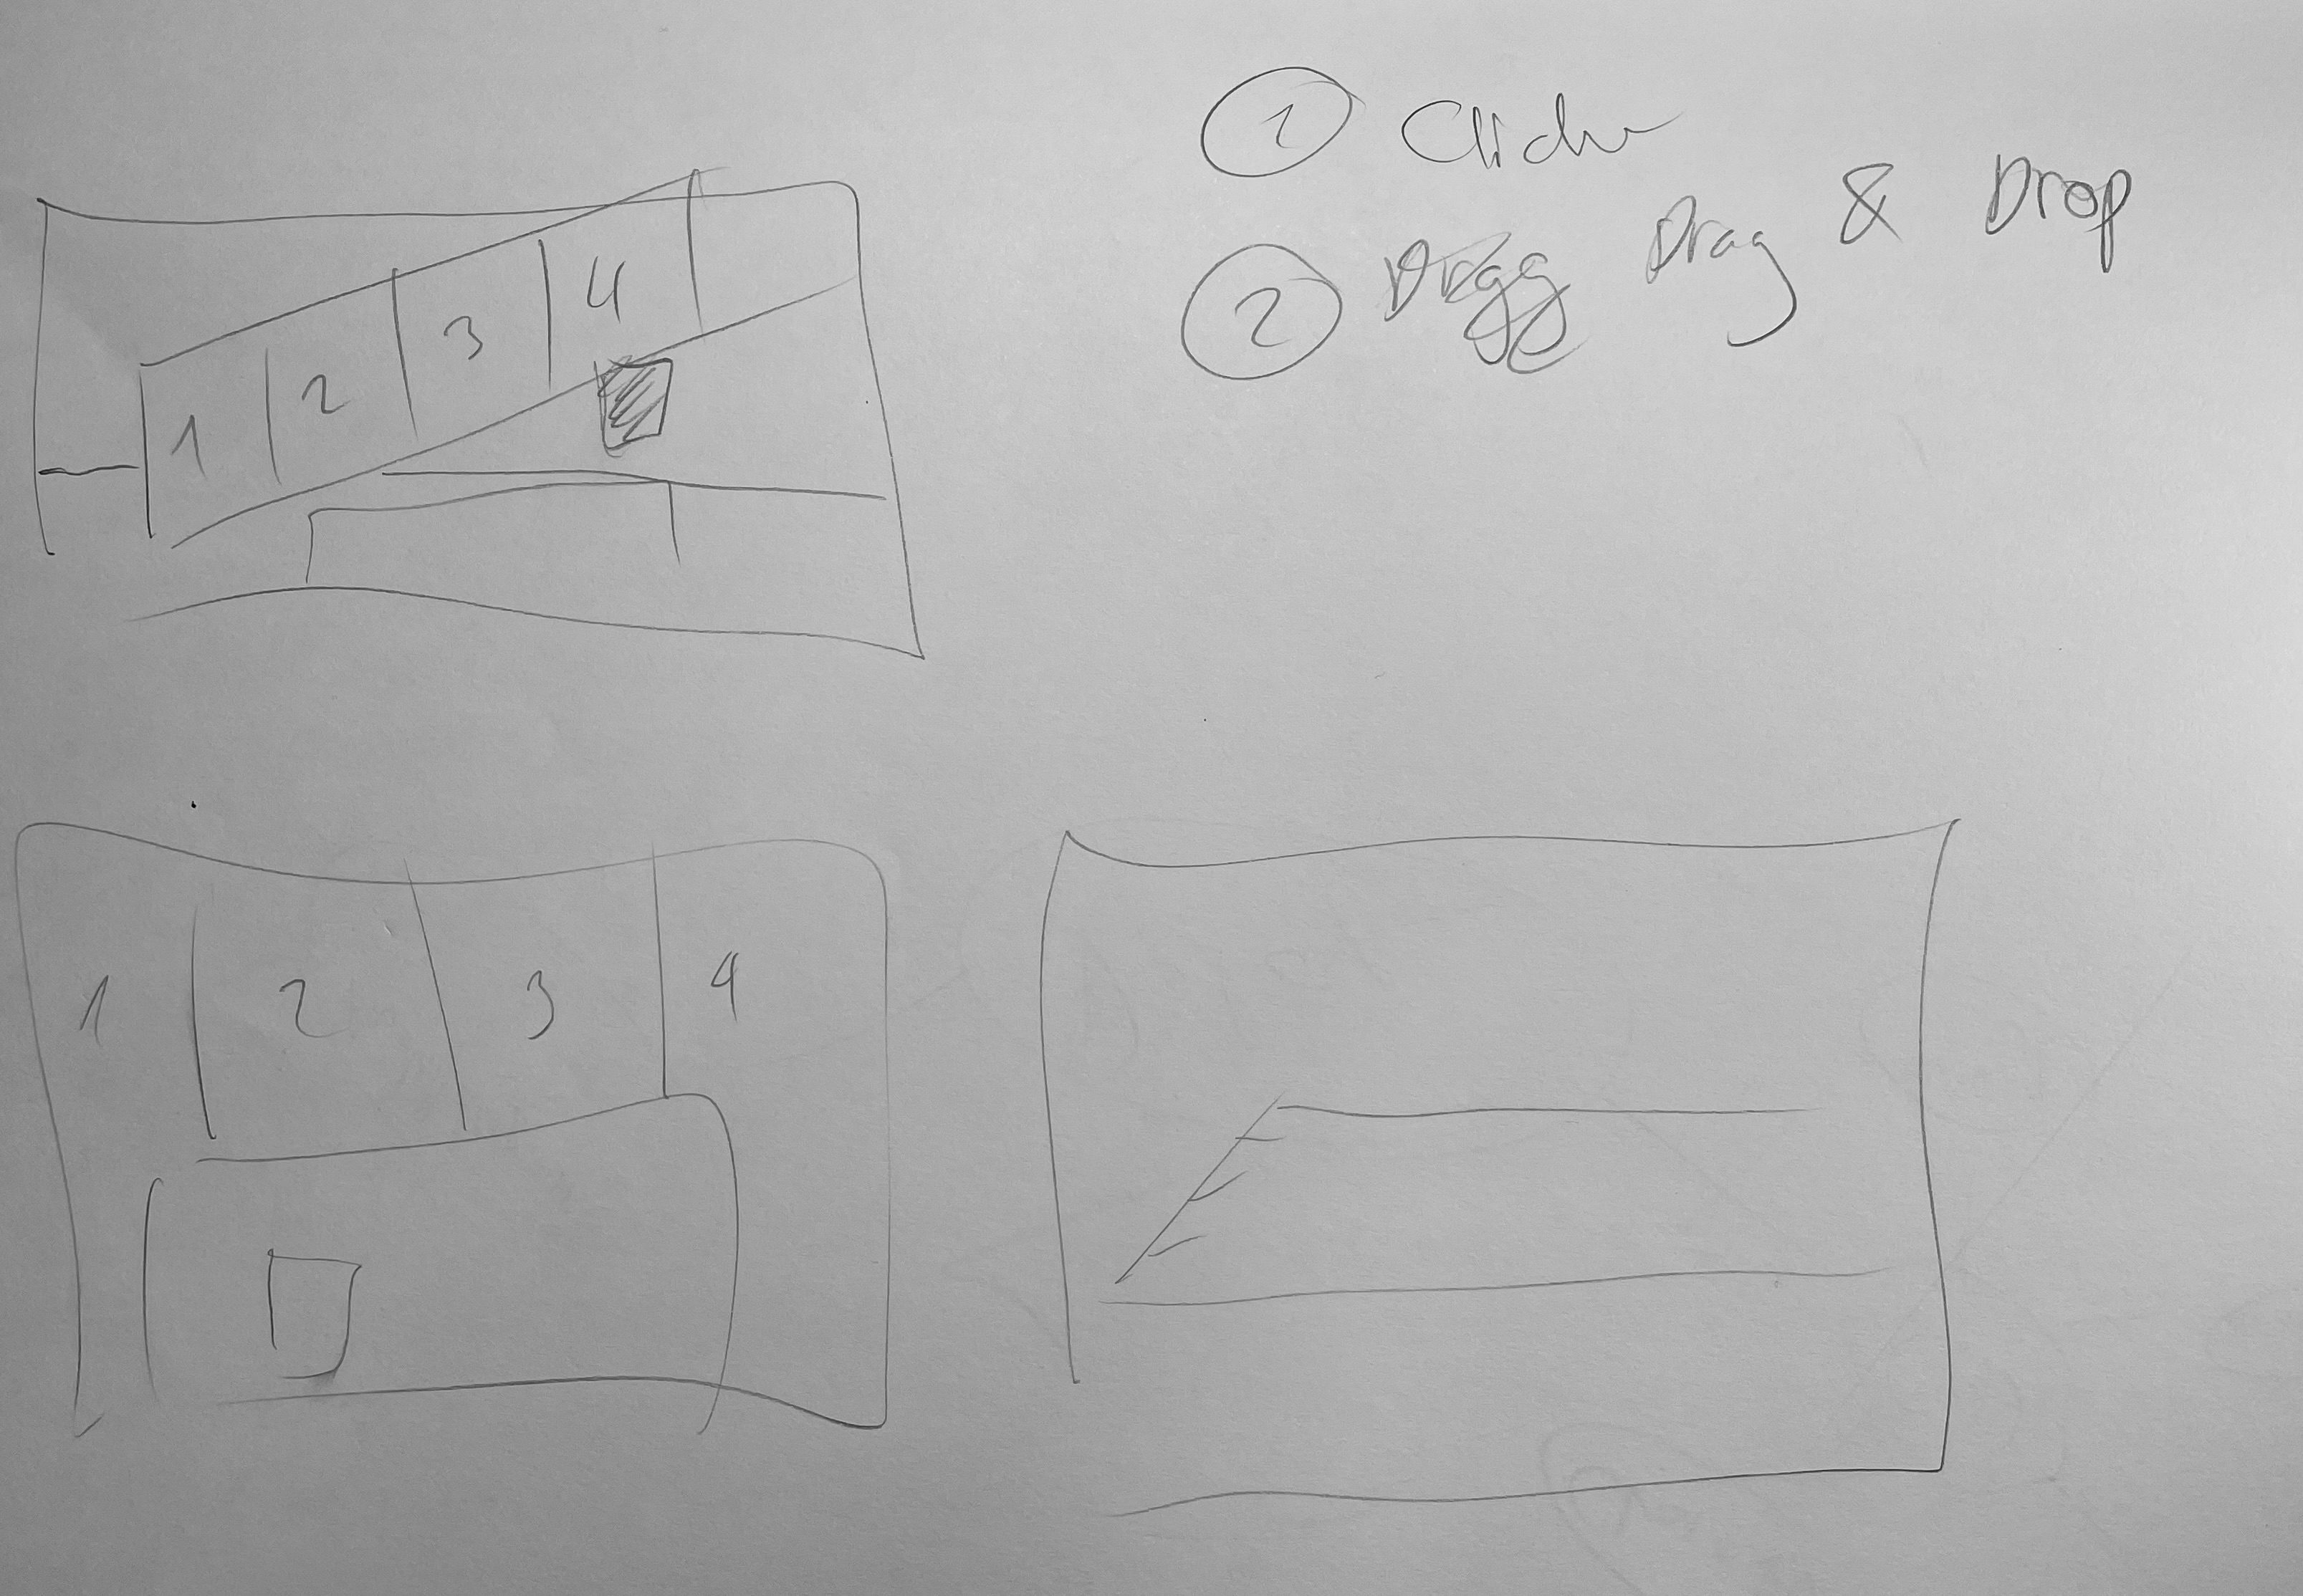
\includegraphics[width=14.5cm]{resources/Sk_dragndrop.jpeg}\\
        \caption{Mechanik der Karten / Spawnen von Truppen}
    \end{figure}

\section{Mindmap}
    \begin{figure}[H]
        \centering
        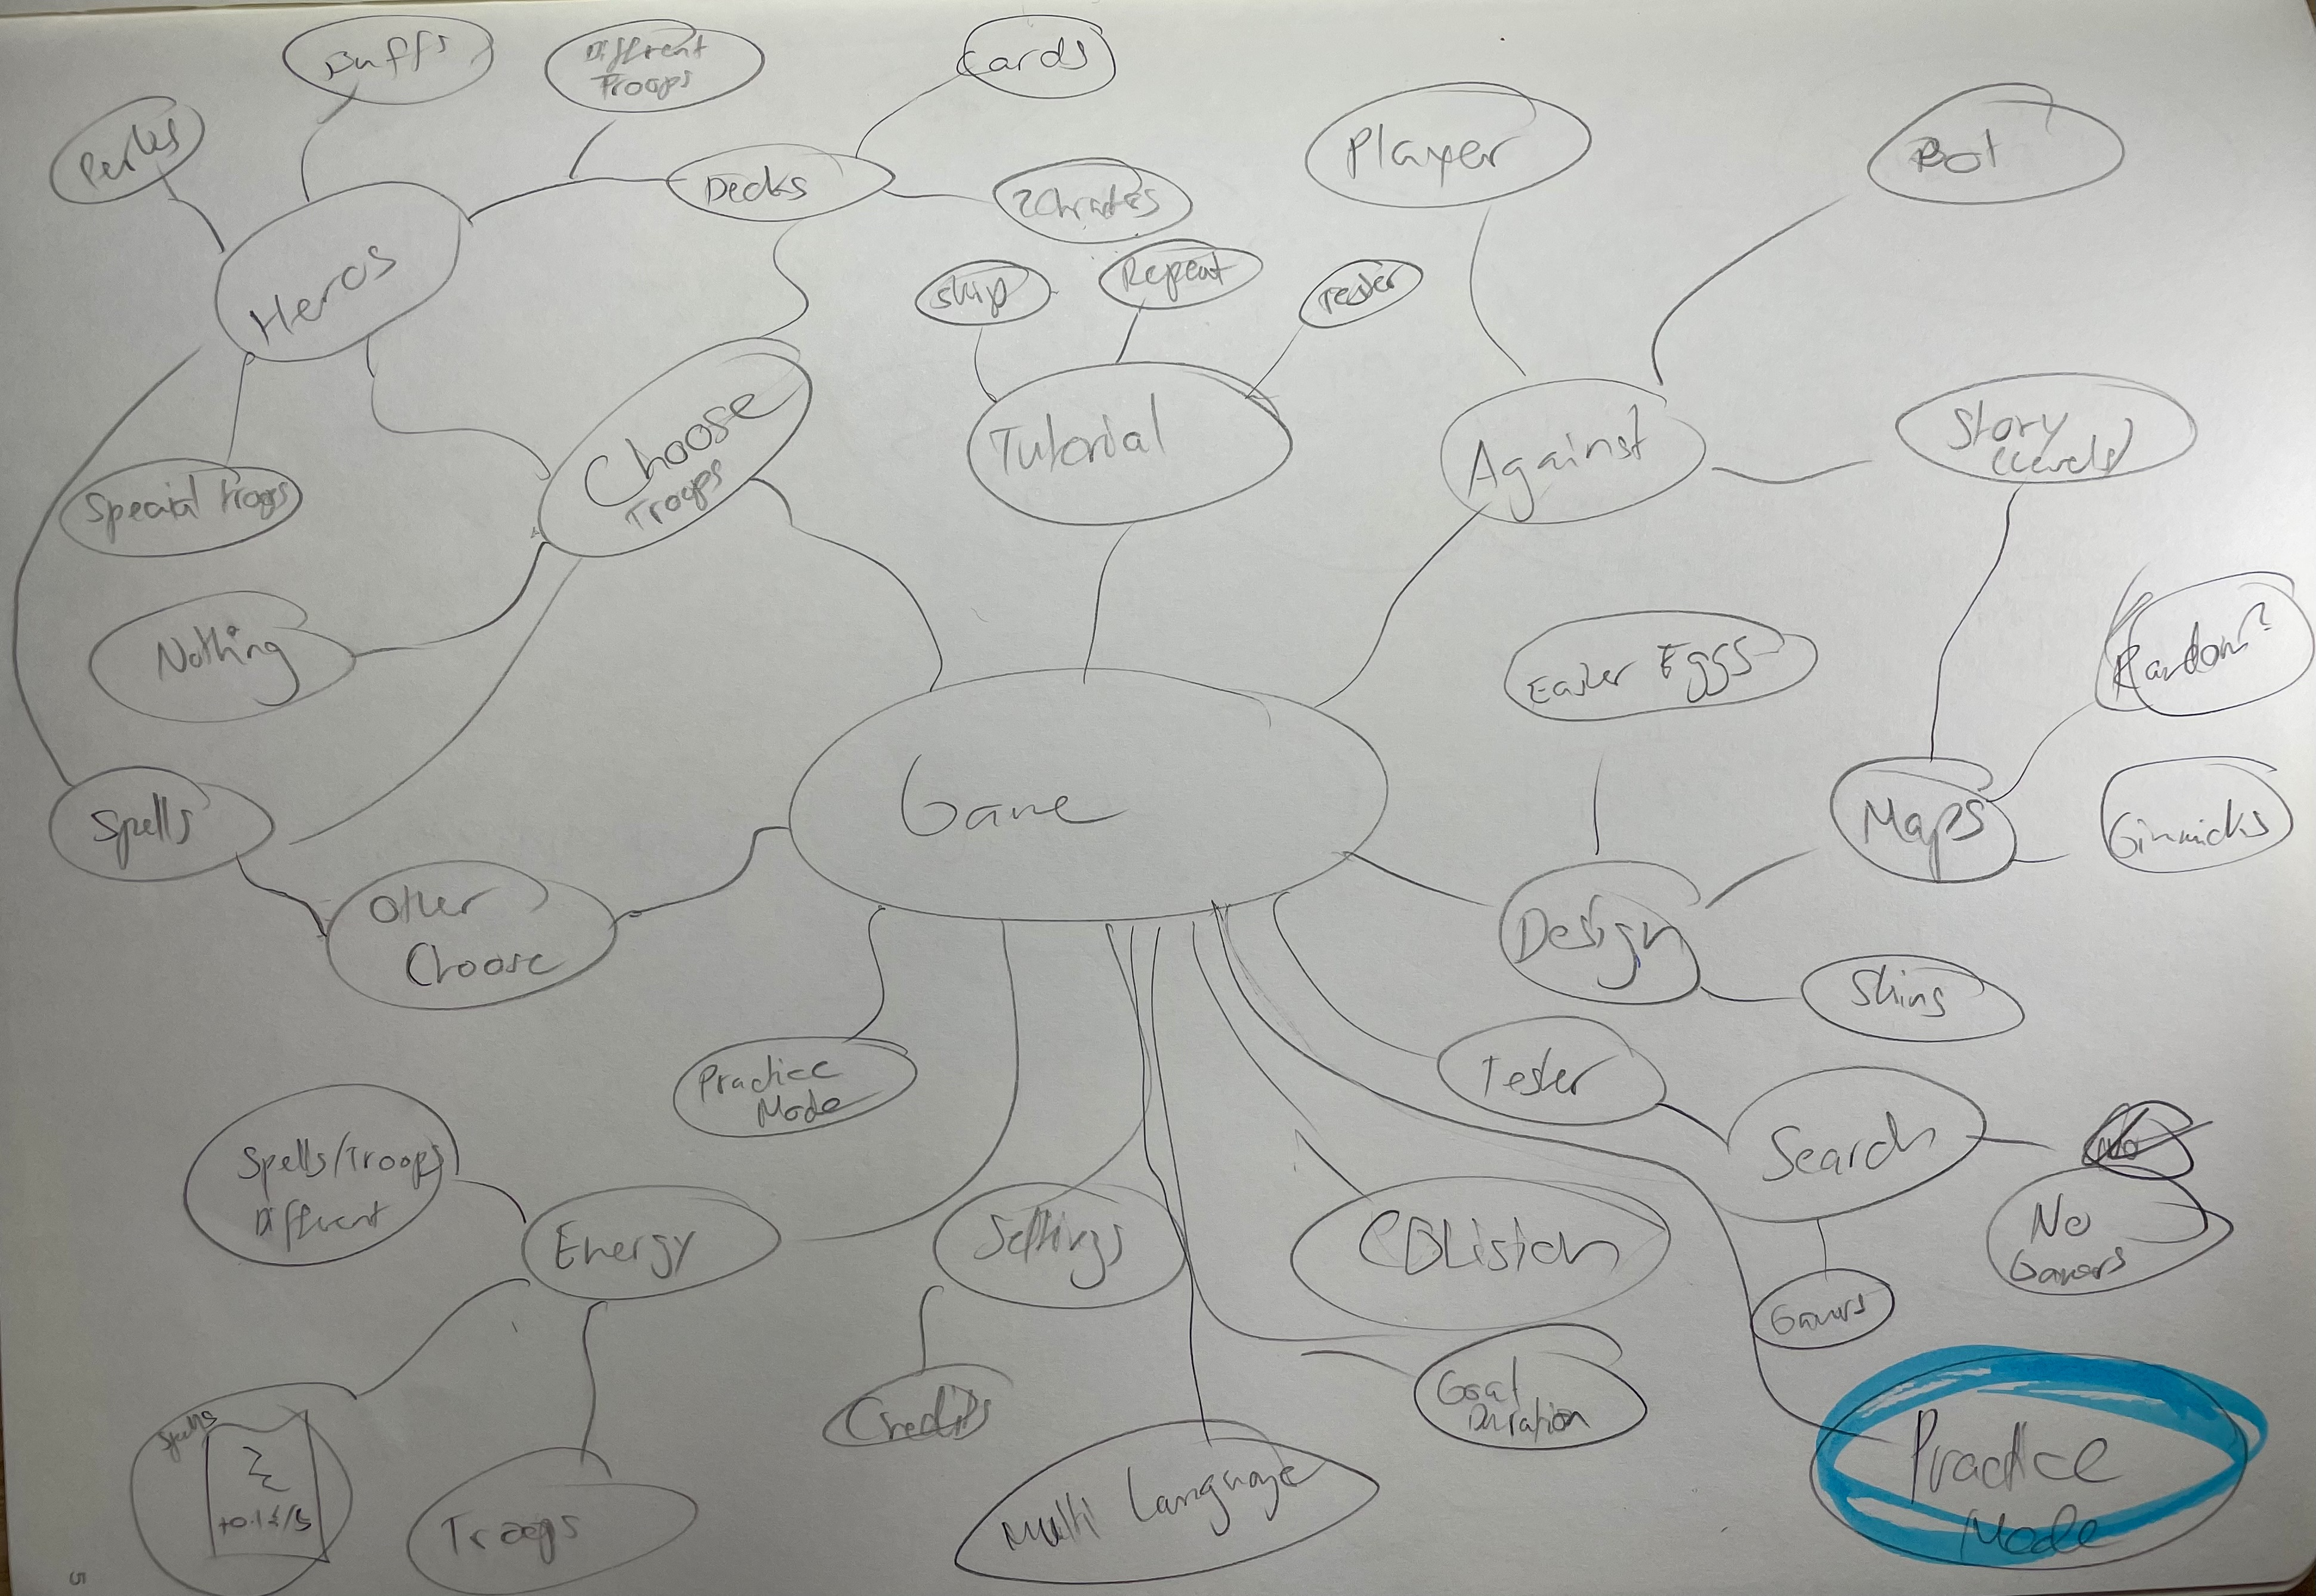
\includegraphics[width=14.5cm]{resources/Sk_mindmap1.jpeg}\\
        \caption{Mindmap}
    \end{figure}


\section{Überlegungen zum Spielprinzip}

Die Idee des Spielprinzips wird im folgenden Unterkapitel grob beschrieben.\
\begin{itemize}
    \item In unserem Spiel treten zwei Spieler*innen gegeneinander an. Dabei befinden sich die Startbereiche der Spieler*innen auf der linken bzw. rechten Seite einer steinernen Brücke.
    \item In die Schlacht begleitet wird jede*r Spieler von vier Helden. Diese Helden schreiten zu Beginn des Spieles durch die magischen Portale und bilden einen ersten Verteidigungswall.
    Sterben jene Helden, lösen sie einen Zauber aus, der alle gegnerischen Truppen auf dieser Linie der Brücke ausradiert.
    \item Der*die Spieler*in kann zudem Unterstützung aus dem eigenen Lager befehligen. Die verfügbaren Truppen erhält der*die Spieler*in in Form von Karten. Der*die Spieler*in kann mit der Verschiebung dieser Karten auswählen, durch welches Portal sie schreiten sollen.
    \item Jede Truppe verlangt eine unterschiedliche Menge an Kraft (Mana, spirituelle Energie), um das Portal zu durchschreiten. Die zur Verfügung stehende Mana wird oben recht angezeigt.
    \item Nach jeder Durchschreitung muss der*die Spieler*in eine bestimmte Zeit warten, bis er die nächste Truppe auswählen kann.
    \item Gelingt es einer verbündeten Einheit das gegnerische Portal zu durchschreiten, ist das Spiel vorbei und man hat gewonnen. 
    \item Mit den Pfeiltasten kann der*die Spieler*in steuern, welchen Teil des Schlachtfelds er überblicken will.
\end{itemize}



% \includegraphics[width=\textwidth]{resources/diagrams/domain-model}

\chapter{Anforderungen}

\section{KZO}
% \includegraphics[height=18cm]{resources/diagrams/use-case}
Die Anforderungen der Schule halten sich in Grenzen. Zum einen gibt es fast keine
genauen Anforderungen und die Anforderungen, die es gibt, sind relativ tief gehalten. Die drei Anforderungen der KZO sind:
\begin{enumerate}
    \item \textbf{Zeit} \\
        Geplant ist ungefähr eine Lektion pro Woche, denn diese wir dem Stundenplan für das Semester abgezogen.
        Jedoch ist diese Anforderung bei uns nicht relevant, denn unser Projekt ist eine riesige Maturitätsarbeit.
        Wir werden ohne Probleme diese Zeitanforderung erreichen und auch bei Weitem überschreiten.
    \item \textbf{Begleitperson} \\
        Jede Maturitätsarbeit braucht eine Begleitperson. Also eine Lehrperson, welche die Arbeit bewertet und einen unterstützt.
        Letzteres, also Unterstützung, war bei uns sehr schwierig, denn keine Lehrperson kennt sich mit Unity und C\# genug gut aus.
        Wir sind bereits früh auf Herrn Kern, ein Informatiklehrer, zugegangen.
        Er hat uns an Martin Hunziker, Leiter der IT, weitergeleitet. Dieser nahm uns sehr gerne auf, mit der Anmerkung, dass unsere Arbeit sehr schwierig sein wird, umzusetzen.
    \item \textbf{Plagiat} \\
        Arbeiten dürfen nicht einfach kopiert werden. Wir haben uns zwar bei gewissen Problemen online inspirieren lassen, jedoch sind diese keine Plagiate.
        Der grösste Teil unseres Codes und alles unserer schriftlichen Arbeit sind von uns geschrieben.
\end{enumerate}

\section {Unsere eigenen Anforderungen}
Gewisse Features sind für das Funktionieren des Spiels wichtiger als andere.
Zum Beispiel sind Einstellungen, Truppen und Multiplayer notwendiger als die Monetarisierung, zumindest nach unserer Ansicht.
Deshalb ist dieser Abschnitt in 4 Gruppen unterteilt:
\begin{enumerate}
    \item \textbf{Notwendig:}
        Ohne diese Features läuft das Spiel nicht oder ist sehr mangelhaft,
        voller Fehler und unspielbar. Ohne diese Features ist Idee des Spieles nicht erkennbar.
    \item \textbf{Anvisiert:}
        Diese Features sind unser Ziel. Sie wurden Herr Hunziker, also der Begleitperson, angekündigt und sind alle in einem Plan festgehalten.
        Diese Ziele sollen dazu führen, dass das Spiel
        gut spielbar ist und es Spass macht. Sie sind auch dafür essenziell, das Spiel nicht zu monoton zu gestalten und sollten
        alle bis zum Abgabetermin der schriftlichen Arbeit vollendet sein.
    \item \textbf{Möglichkeiten:}
        Möglichkeiten das Spiel noch auf die Spitze zu bringen. Keine dieser Anforderungen ist nötig
        für das Spielen, jedoch können sie das Spielerlebnis spannender und ausgereifter machen. Diese
        Ziele sind entweder in den Sternen geschrieben oder zu erreichen bis zur mündlichen Präsentation.
        Vereinzelt können diese, wie die anvisierten Anforderungen, noch bis zur schriftlichen Abgabe erreicht werden.
    \item \textbf{Verworfen:}
        Weitere Ideen, welche wir hatten, jedoch als unmöglich oder nicht sinnvoll erachten.
\end{enumerate}

\subsection*{Notwendig}
\begin{itemize}
    \item \textbf{System} \\
        Unser Spiel sollte auf den meisten modernen Geräten funktionieren. Es soll auf macOS und
        Windows fliessend gespielt werden können. Also mit mindestens 60FPS.
    \item \textbf{Benutzeroberfläche} \\
        Eine Startseite mit einem ''Spielen''-Knopf, einem ''Einstellungen''-Knopf, einem
        ''Credits''-Knopf und einem ''Verlassen''-Knopf. Sie soll intuitiv sein und einigermassen
        schön aussehen. Die Benutzeroberfläche soll mit Touch bedienbar sein, andere Eingabemöglichkeiten
        werden nicht unterstützt.
    \item \textbf{Lokaler Multiplayer} \\
        Das Spiel soll im lokalen Netz gespielt werden können. So zum Beispiel mit Freunden oder Familie.
        Es sollte mithilfe der IP-Adresse innerhalb des gleichen Netzes zusammengespielt werden können.
    \item \textbf{Einstellungen} \\
        Auflösung, Vollbild und Lautstärke müssen eingestellt werden können.
    \item \textbf{Kamera} \\
        Die Kamera ist beweglich und das ganze Schlachtfeld ist sichtbar.
    \item \textbf{Truppen} \\
        Es braucht Truppen, die für einen kämpfen können. Diese sind notwendig für den Verlauf des Spieles
        und ohne sie hat das Spiel keinen Sinn.
    \item \textbf{Gewinnmöglichkeit} \\
        Eine Chance das Spiel zu gewinnen oder verlieren und es somit zu beenden. Dies kann sehr simpel
        mit einer Linie vollendet werden, welche beim Überschreiten das Spiel beendet.
    \item \textbf{Lanes} \\
        Unser Spiel ist zwar 2.5D, aber hat dennoch eine Tiefe.
    \item \textbf{Synchronisation} \\
        Unser Spiel soll in Echtzeit spielbar sein, deswegen müssen die beiden Spieler Synchronisiert das Gleiche sehen. Eine De-Synchronisation wäre verheerend. 
    \item \textbf{Crossplay}
        Die Möglichkeit sich mit einem Windows Rechner und einem macOS Rechner zu verbinden und zusammenzuspielen.
\end{itemize}

\subsection*{Anvisiert}
\begin{itemize}
    \item \textbf{Helden} \\
        Beide Spieler haben eine Art Truppe, welche ihre Siegeslinie beschützt. Sie haben einen Racheeffekt, welcher die
        Lane ausradiert, damit das Spiel nicht sofort vorbei ist.
    \item \textbf{Design} \\
        Das Spiel sollte vom Aussehen her was hergeben. Es sollte nicht wie ein Prototyp, sondern wie ein 
        vollendetes Spiel aussehen. 
    \item \textbf{Deck} \\
        Zu Beginn Spieler könne ihr eigenes Deck aus einer Auswahl von Karten zusammenstellen. Im Spiel werden davon per Zufall Karten gezogen.
    \item \textbf{Bot} \\
        Ein sehr simpler Algorithmus um alleine gegen den Computer zu spielen auf den Schwierigkeitsstufen \textit{'Einfach', 'Mittel', 'Schwierig'}.
        Es sollen rein zufällig Truppen geschickt werden, bei höherer Schwierigkeit mehr.
    \item \textbf{Truppen}
    \begin{itemize}
        \item \textbf{Nahkampf}
            Eine Truppe mit wenig Reichweite.
        \item \textbf{Fernkampf}
            Eine Truppe die auf Reichweite angreift. Sie schiesst Projektive, zum Beispiel ein Bogenschütze,
            der mit Pfeilen schiesst.
        \item \textbf{Suizid}
            Eine Truppe die bei Berührung mit einem Gegner stirbt und einen Effekt auslöst.
    \end{itemize}
    \item \textbf{Effekte}
    \begin{itemize}
        \item \textbf{Gift:}
            Zeitlich limitierter und wiederholender Schadenseffekt. Eine visuelle Markierung soll vorhanden sein
            und das gleiche Gift, also der gleichen Truppe, soll nur einmal auf jemanden sein.
        \item \textbf{Dornen:}
            Truppen, welche Charaktere mit Dornen attackieren, erhalten schaden. Soll nach Auswahl auf Nahkämpfer,
            Fernkämpfer oder beides wirken.
        \item \textbf{Rache:}
            Truppen mit Rache haben einen Effekt nach ihrem Tod. Zum Beispiel eine Truppe beschwören oder Schaden verursachen.
    \end{itemize}
\end{itemize}

\subsection*{Möglichkeiten}
\begin{itemize}
    \item \textbf{Zauber} \\
        Als Alternative sollen nicht alle Karten einfach eine Truppe herbeirufen. Gewisse Karten sollten nur einen Effekt auslösen.
        Beispiele für Zauber:
            "Heile deine Helden um 5 leben"
            "Gib deinen Helden 5 Rüstung"
            "Verursache allen gegnerischen Truppen 5 Schaden"
            "Ziehe 3 Karten"
    \item \textbf{Monetarisierung} \\
    Hierfür sind uns drei Möglichkeiten eingefallen, hier jeweils die Vor- und Nachteile:
    \begin{enumerate}
        \item \textbf{Kaufbare Gegenstände}
        \begin{itemize}
            \item[+] Vielseitige und Nachhaltige Monetarisierung. Neue Features, bedeuten auch neue Geldmöglichkeit. Die Inhalte sollten
                     auch erspielbar sein, somit kann bezahlen zwar zu Vorteilen führen, jedoch mit viel Spielen trotzdem erreichbar sein.
            \item[-] Pay-to-Win
        \end{itemize}
        \item \textbf{Skins}
        \begin{itemize}
            \item[+] Weit verbreitet und sehr beliebt bei Spielern. Gibt keinem Spieler Vorteile
            \item[-] Wenig Nutzen und sehr aufwändig. Neue Designs zu erstellen, wäre bei uns nicht so sinnvoll.
                     Wir haben noch sehr viel Features zu implementieren und sind nicht Designer. Für uns braucht es sehr
                     viel Zeit eine brauchbare Darstellung zu erstellen und der Mehrwert, welcher dem Spiel beigetragen wird, ist marginal.
        \end{itemize}
        \item \textbf{Kostenpflichtiges Spiel}
        \begin{itemize}
            \item[+] Einmalige Bezahlung, was für viele Nutzer lukrativer ist. Jedoch gilt dies vor allem bei Singleplayer Spielen.
            \item[-] Wir nehmen an, dass wenige Leute bereit wären, Geld für unser Spiel zu bezahlen.
                    Dafür wird es nicht genug ausgereift sein.
                    Auch ist diese Methodik nicht nachhaltig und führt nur zu einer einmaligen Geldspritze.
                    Viele grössere Spiele führen deshalb später
                    DLCs ein, um das Spiel zu erweitern.
                    Jedoch ist dies bei einem Multiplayer Spiel Pay-to-Win.
                    Abschliessen müssten wir höchstwahrscheinlich selbst Geld vorauswerfen, um unser Spiel anbieten zu können, z.B. auf Steam.
        \end{itemize}
        
    \end{enumerate}
    \item \textbf{Helden} \\
        Eine Auswahl von Helden, mit unterschiedlichem Schaden, Leben und Effekten, würde das Spiel nochmals spannender machen. Auch sollten gewisse Truppen auf bestimmte Helden limitiert sein. 
    \item \textbf{Design} \\
        Wenn die Zeit vorhanden ist, kann das Design immer verbessert werden. Hier gehts es aber um den Feinschliff, z.B. mehr Hintergründe, und mehr Dinge selbst zu designen.
    \item \textbf{Tutorial} \\
        Eine Anleitung für Anfänger wäre sehr schön. Sie soll neuen Spielern das Anfangen erleichtern. Es sollte aber auch überspringbar sein,
        damit alte Spieler, es nicht nochmals spielen müssen. Es soll nicht lange sein und nicht schwierig. Dennoch soll es alle Mechaniken des Spiels
        erklären, am besten Anhand von Gameplay.
    \item \textbf{Truppen}
        Weitere Truppen können jederzeit erstellt werden. Hier ist kein Limit gesetzt. Leben, Schaden, Darstellung, Effekt und vieles mehr kann angepasst werden.
    \item Effekte
    \begin{itemize}
        \item \textbf{Wiederbelebung:}
            Die Truppe wird wiederbelebt, sofort an Ort und Stelle oder mit einer Verzögerung am Startpunkt.
        \item \textbf{Rüstung:}
            Die Truppe hat zusätzlichen zu den Leben auch Rüstung. Die Rüstung wird zuerst abgezogen und hat im Gegensatz zum Leben keine Limite.
        \item \textbf{Aura:}
            Die Truppe fügt gegnerischen Truppen in einem gewissen Radius permanent Schaden zu.
    \end{itemize}
    \item \textbf{Mehrsprachig} \\
        Das Spiel soll in Englisch, Deutsch und Französisch spielbar sein.
    \item \textbf{Ingame-Chatfenster}\\
        Ein Textfeld, in dem man sich mit dem Gegner unterhalten kann.
\end{itemize}

\subsection*{Bereits früh verworfen}
\begin{itemize}
    \item \textbf{Online Multiplayer} \\
        Besser als ein Multiplayer, der limitiert auf dasselbe Netz ist, ist ein Multiplayer, der weltweit verfügbar ist. Jedoch ist von einem Computer auf einen anderen zu
        verbinden dank der Firewall von Router und Computer, nahezu unmöglich. Es würden sich viele weitere Probleme ergeben, wie zum Beispiel Port-Forwarding. Dies ist einer der Gründe, weshalb ein Server sehr praktisch ist. Mit diesem wäre dieses
        Problem gelöst. Server sind aber teuer und aufwändig. 
    \item \textbf{Shop} \\
        Nicht alle Karten sind von Beginn an freigeben, sondern müssen freigespielt werden.
        So kann zum Beispiel eine Ingame Währung erspielt werden und damit im Shop Karten oder sonstige Dinge gekauft werden.
        Der Shop kann mit Zahlungsmethoden ausgestattet werden und so zur eventuellen Monetarisierung beitragen.
    \item \textbf{Kampagne} \\
        Singleplayer gegen bestimmte vorprogrammierte Gegner. Sie sollen immer schwieriger werden und bestimmte Herausforderungen mit sich bringen.
        Bei Vollendung werden Belohnungen verteilt.
    \item \textbf{Anti-Cheat} \\
        Eine sehr komplexe Software um das Schummeln zu verhindern. Ist in allen grösseren Spielen vorhanden. Teilweise sogar auf Systemebene, oder sogar auf Kernel-Level,
        gespeichert und ausgeführt.
    \item \textbf{Errungenschaften} \\
        Eine Übersicht und die Möglichkeit die Errungenschaften zu erfüllen.
        Gegebenenfalls Belohnungen verteilen, wie zum Beispiel bestimmte Karten freischalten.
        Diese Erweiterung ist keines Falls notwendig und ein absolutes nice-to-have Feature.
\end{itemize}

% \includegraphics[height=10cm, width=\textwidth]{resources/mockups/mockup-login}
\chapter{Risikoanalyse}
Wir haben mögliche Risiken in verschiedene Stufen eingeteilt.
Die Einstufung geschah basierend auf der Eintrittswahrscheinlichkeit (unwahrscheinlich, wahrscheinlich, sehr wahrscheinlich) und Auswirkung (unbedenklich, kritisch). 
Um das Risiko zu managen, haben wir für jedes Risiko eine Reduktionsstrategie definiert.\\
In den folgenden Teilkapiteln dokumentieren wir die identifizierten Risiken nach folgendem Schema:\\
\\
- Risiko (Eintrittswahrscheinlichkeit und Auswirkung)
\begin{enumerate}
    \item Reduktionsstrategie: Strategie um die Wahrscheinlichkeit und/oder die Auswirkung zu reduzieren.
    \item Reduziertes Risiko: Risiko nach der Umsetzung der Reduktionsstrategie.
    \item Tatsächliches Outcome: Das tatsächliche Endresultat
\end{enumerate}

\section{Hoch}
\begin{enumerate}
    \item Vergange Maturitätsarbeiten, die ein Videospiel als Ziel hatten, sind gescheitert (Wahrscheinlich und Kritisch)
    \begin{enumerate}
        \item Reduktionsstrategie: Klare Anforderungsspezifikation, Planung und Aufteilung der Arbeitspakete, laufende Überprüfung der Planung/Zielerreichung, regelmässiger gegenseitiger Austausch zum Fortschritt,
        Bereitschaft den empfohlenen Zeitaufwand massiv zu überschreiten.
        \item Reduziertes Risiko: Die Eintrittswahrscheinlichkeit ist reduziert. Beim Eintreten ist der Erfolg der Arbeit allerdings immer noch gefährdet.
        \item Tatsächliches Outcome: Risiko nicht eingetreten. Maturitätsarbeit mit funktionierendem Videospiel fertiggestellt.
    \end{enumerate}

    \item Beide Teammitglieder haben keine Ahnung von der Entwicklung eines netzwerkfähigen Multiplayer-Spiels (Wahrscheinlich und Kritisch)
    \begin{enumerate}
        \item Reduktionsstrategie: Erstellen der grundsätzlichen Multiplayerfunktionalität in einer einzelnen Spielinstanz, danach Ausbau auf mehrere Spielinstanzen über das lokale Netzwerk (Host und Client)
        \item Reduziertes Risiko: Spiel am selben Rechner ist sehr wahrscheinlich möglich, primäres Ziel der Arbeit ist auch ohne Netzwerkfähigkeit erfüllt.
            Das Risiko ist reduziert immer noch sehr hoch.
            Wir haben uns beide an Multiplayer fest gefressen und werden es höchst wahrscheinlich trotzdem umsetzen
        \item Tatsächliches Outcome: Risiko nicht eingetreten. Mehrere Spieler können übers Netz zusammen spielen, Ziel nur mit beträchtlichem Aufwand erreicht (1/3 der gesamten Entwicklungszeit).
    \end{enumerate}

    \item Spiel enthält unentdeckte / unbekannte Fehler die den Spielspass verderben (Wahrscheinlich und Kritisch)
    \begin{enumerate}
        \item Reduktionsstrategie: So viel testen wie möglich/sinnvoll, Bugs kategorisieren, sich auf kritsche Bugs konzentrieren, Code Reviews
        \item Reduziertes Risiko: Wir schätzen das reduzierte Risiko immernoch als hoch ein, da selbst wenn die Eintritswahrscheinlichkeit stark reduziert ist; kann dieser eine unentdeckte Fehler den ganzen Spielspass vermiesen.
        \item Tatsächliches Outcome: Nach Abschluss der Alpha Testphase sind keine Fehler bekannt. Wir drücken nun die Daumen, dass Herr Hunziker keine Bugs findet.
    \end{enumerate}

\end{enumerate}

\section{Mässig}
\begin{enumerate}
    \item Elia hat noch nie mit Unity gearbeitet (Sehr wahrscheinlich und Unbedenklich)
    \begin{enumerate}
        \item Reduktionsstrategie: Elia befasst sich zu Beginn mit Unity, Marc hat Vorwissen und kann Elia unterstützen
        \item Reduziertes Risiko: Falls Elia auf Schwierigkeiten stösst, kann dies zu zeitlichen Mehraufwand führen.
        \item Tatsächliches Outcome: Risiko nicht eingetreten. Elia konnte alles Nötige zu Beginn erlernen, Probleme durch Internetrecherchen klären oder Marc fragen. 
    \end{enumerate}
\end{enumerate}

\section{Tief}
\begin{enumerate}
    \item Wir werden selbst nicht mit unserem Spiel zufrieden sein. (Wahrscheinlich und Unbedenklich)
    \begin{enumerate}
        \item Reduktionsstrategie: Sich bewusst sein, dass wir nur zwei Schüler sind, die keine bisherigen Erfahrungen hatten. Wir dürfen uns nicht an etwas ''festfressen''.
        \item Reduziertes Risiko: Realistische Erwartungshaltung
        \item Tatsächliches Outcome: Basierend auf der uns zu verfügungsstehenden Zeit und unserem Wissen, sind wird zufrieden mit unserem Produkt. Es gibt immer noch Dinge, die wir gerne verbessern und hinzufügen würden. So könnten wird noch Tausende Stunden investieren.
    \end{enumerate}
\end{enumerate}

\part{Produkt}
\chapter{Resultat}
Kurz gesagt: Wir konnten fast alle unsere Anforderung erfüllen.

\section{Maturitätsarbeit}
% \includegraphics[height=18cm]{resources/diagrams/use-case}
\begin{enumerate}
    \item \textbf{Zeit} \\
        Geplant war ungefähr eine Lektion pro Woche. Wir haben die geschätzten 100 Stunden (50 Stunden pro Person) um den Faktor drei überschritten. Unser gemessener Zeitaufwand während des aktiven Programmierens
        beträgt über 330 Stunden. Hier sind die Stunden, in denen wir uns in der Schule über das Projekt unterhalten haben, nicht notiert.
    \item \textbf{Begleitperson} \\
        Wir hatten glücklicherweise kein Problem eine Begleitperson zu finden. Martin Hunziker war gerne bereit, unsere Arbeit im Blick zu behalten.
    \item \textbf{Plagiat} \\
        Einige Grafiken sind zwar aus dem Internet, jedoch sind alle nutzungsfrei. Wir haben keinen Code geklaut und verwendet. 
\end{enumerate}

\section{Spiel}
In den folgenden Teilkapiteln wird die Erfüllung der in \autoref{chap:foo} gestellten Anforderungen gruppiert dargestellt. 
\subsection{Notwendig}
    \begin{itemize}
    \item \textbf{Systemanforderungen} \\
        Unser Spiel funktioniert sowohl auf macOS als auch auf Windows. Es läuft zudem mit einer FPS von 300, bis teilweise 500, bei den meisten modernen Rechnern.
    \item \textbf{Benutzeroberfläche} \\
    \begin {itemize}
        \item \textbf{Startseite} \\
            Unsere Startseite hat einen ''Spielen''-Knopf, einen ''Einstellungen''-Knopf, einen ''Credits''-Knopf und einen ''Verlassen''-Knopf. Unsere Tester bewerteten die Startseite
            als intuitiv verständlich. Bedienbar mit der Maus, hatten die Tester keine Probleme sich zurechtzufinden.
            \begin{center}
                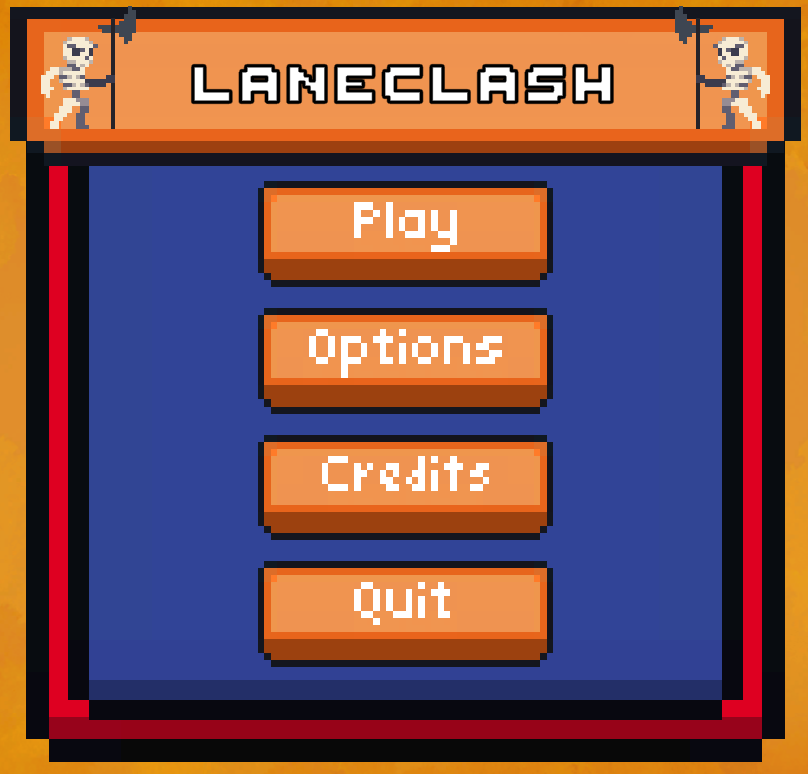
\includegraphics[height=7cm]{resources/laneclash.png}\\
            \end{center}

        \item \textbf{Credits}\\
            Es gibt die Möglichkeit, die Credits vorzeitig zu verlassen. Dies geschieht durch das Drücken des Hausbuttons. Die Tester fanden dies auch sehr intuitiv.
            \begin{center}
                \includegraphics*[width = 7cm]{resources/credits.png}\\
            \end{center}
            
        \item \textbf{Settings}\\
            Man kann hier die Auflösung ändern und auswählen, ob das Spiel als Vollbild dargestellt werden soll. Auch gibt es hier die Möglichkeit, die Musik lauter oder leiser zu stellen
            oder zu muten. Wenn man Einstellungen geändert hat, muss man das Speichern bestätigen. 
            \begin{center}
                \includegraphics*[height=7cm]{resources/setting.png}\\
            \end{center}
            Nach Bestätigung der Änderung der Auflösung, werden die Änderungen angewendet und man hat zehn Sekunden Zeit erneut zu bestätigen. Sonst werden die Änderungen zurückgesetzt.
            Dies wurde implementiert, um eventuellen Problemen vorzubeugen. 
            \begin{center}
                \includegraphics*[height=3cm]{resources/resolution.png}\\
            \end{center}
            
        \item \textbf{Server Management}\\
            Nach Bedienung des ''Start''-Knopfs gibt es die Möglichkeit, einen Server zu hosten oder einer bereits existierenden Lobby als Client beizutreten. Ausserdem kann man
            automatisch nach bereits existierenden Servern suchen.
            \begin{center}
                \includegraphics*[height = 3cm]{resources/server.png}\\
            \end{center}
            Den Server kann man mit einem Linksklick auswählen.
            \begin{center}
                \includegraphics*[width=6cm]{resources/discovered.png}\\
            \end{center}
            
        \item \textbf{Lobby Management}\\
            Player (1) ist dabei immer der Host, und Player (2) immer der Client. Das eigentliche Spiel beginnt erst, sobald beide Spieler bereit, also ''ready'', sind. 
            Der Status ''ready'' wird dabei immer aktualisiert dargestellt. Der Host hat ausserdem die Möglichkeit, den Spieler (2) aus der Lobby zu entfernen. 
            \begin{center}
                \includegraphics*[width = 5cm]{resources/lobby.png} \includegraphics*[width=5cm]{resources/lobbyc.png}\\ 
            \end{center}
            
        \item \textbf{InGame-UI}\\
            Der Host hat die Möglichkeit, das Spiel zu beenden. Er kann auch direkt aufhören zu hosten. 
            Auch der Client hat durchgehend die Möglichkeit, den Server zu verlassen.
            \begin{center}
                \includegraphics*[height=2cm]{resources/returnlobby.png} \includegraphics*[height=2cm]{resources/stopclient.png}\\
            \end{center}
            Im Pausenmenu kann man ausserdem leicht die Musiklautstärke und die Stärke des Schneefalls ändern. Dieses Menu kann mit ESC geöffnet und geschlossen werden.
            \begin{center}
                \includegraphics*[height=2cm]{resources/pause.png}\\
            \end{center}
            
            


    \end {itemize}

    \item \textbf{Lokaler Multiplayer} \\
        Das Spiel kann im lokalen Netz gespielt werden. Zum Testen kann man das Spiel auch zweimal parallel auf demselben Gerät laufen lassen. Als Protokoll haben wir TCP gewählt.
        Folgende vier Punkte waren entscheidend für die Wahl von TCP gegenüber UDP:
        \begin{itemize}
            \item \textbf{Zuverlässigkeit}\\
                Es gibt keine Probleme mit verloren gegangenen Paketen. Ging ein Paket verloren, sendet TCP es einfach erneut. Entweder werden alle Daten erfolgreich übermittelt,
                oder es folgt eine Errormeldung.
            \item \textbf{Sequenziert}\\
                TCP stellt sicher, dass jede Nachricht in der gleichen Reihenfolge eintrifft, in der sie gesendet wurde. Wenn man ''a'' vor ''b'' sendet, erhält man auf der
                anderen Seite garantiert auch zuerst ''a'' und dann ''b''.
            \item \textbf{Verbindungsorientiert}\\
                TCP hat sich auf das Konzept einer Verbindung spezialisiert. Eine Verbindung bleibt so lange geöffnet, bis entweder der Client oder der Server sich dazu entscheiden, sie zu schliessen.
                Anschliessend werden sowohl Client als auch Host benachrichtigt, dass die Verbindung beendet wurde.
            \item \textbf{Überlastungskontrolle} \\
                Wenn ein Server überlastet wird, drosselt TCP selbstständig die Daten, um einen Zusammenbruch durch Überlastung zu verhindern.


        \end{itemize}
    \item \textbf{Einstellungen} \\
        Auflösung, Vollbild, Lautstärke und Stärke des Schneefalls können eingestellt werden.
    \item \textbf{Kamera} \\
        Die Kamera ist beweglich und das ganze Schlachtfeld ist sichtbar. Mit den Pfeiltasten kann man die Kamera frei bewegen und hinein- bzw. hinauszoomen.
    \item \textbf{Truppen} \\
        IMPORTANT\\
        IMPORTANT\\
        IMPORTANT\\
        IMPORTANT\\
        IMPORTANT\\
        IMPORTANT\\
        IMPORTANT\\
        IMPORTANT\\
        IMPORTANT\\
        IMPORTANT\\
        IMPORTANT\\
        IMPORTANT\\
        IMPORTANT\\
        IMPORTANT\\
        IMPORTANT\\
        IMPORTANT\\
        IMPORTANT\\
    \item \textbf{Spielende} \\
        Um zu gewinnen, muss eine eigene Truppe die Portale des Gegners durchschreiten. Dies verhindern zuerst sogenannte Helden. Sterben jene Helden, erledigt ihr Racheeffekt alle
        Truppen, die sich auf jener Linie des Helden befanden.
    \item \textbf{Lanes} \\
        Unser Spiel hat vier sogenannte Linien (''Lanes''). Diese unterschiedlichen Linien wurden in der Tiefe nach hinten verschoben. Der Spieler hat die Auswahl, in welcher Reihe er seine Truppen auf den Gegner zuschicken will.
    \item \textbf{Synchronisation} \\
        Unser Spiel synchronisiert alle Daten in Echtzeit. Dadurch sehen alle Spieler immer dasselbe. Wird der Client aus einem unbekannten Grund disconnected, kann er versuchen,
        sich erneut zu verbinden, und der Server wird dann direkt alle Daten synchronisieren. Auch hier hilft uns das gewählte Protokoll TCP. Geht ein Paket verloren, wird es automatisch
        erneut gesendet. Dies hilft uns dabei, die Synchronisation zu jeder Zeit aufrechtzuerhalten.
    \item \textbf{Crossplay}
        Es ist möglich, sich mit einem Windows Rechner und einem macOS Rechner zu verbinden. Allerdings muss dem Spiel dazu die Kommunikation durch die Firewall teilweise erlaubt sein.
        Bei einer eher aggressiveren Firewall wird zudem teilweise der Server-Broadcast geblockt. Dies hätte zur Folge, dass man die Server nicht automatisch finden kann. 
        Verbinden kann mich sich allerdings trotzdem noch.   
\end{itemize}

\subsection{Anvisiert}
\begin{itemize}
    \item \textbf{Helden} \\
        Beide Spieler haben bei unserer aktuellen Version den gleichen Heldentyp. Dies ist ein magischer Turm. Er hat keine Angriffsmöglichkeiten. Allerdings kann er sich passiv heilen und so als eine
        temporäre Grenze zwischen den gegnerischen Truppen und den eigenen Portalen agieren. Die eigenen Truppen werden durch diese Portale hinter den Helden gespawned.
    \item \textbf{Design} \\
        Wir haben uns für ein 2.5d Design entschieden. Der Vorteil ist, dass wir 2d Grafiken benutzen können. Die Sprites werden dabei um 45 Grad gedreht. Auch 
        die Kamera schaut in einem 45 Grad Winkel auf das Geschehen. Dadurch ergibt sich die Illusion einer Perspektive, in der man von der Seite auf das Geschehen schaut. 
        \begin{center}
            \includegraphics*[height=5cm]{resources/25d.png} \includegraphics*[height=5cm]{resources/25dtwo.png}\\
        \end{center}
        
    \item \textbf{Effekte}
    \begin{itemize}
        \item \textbf{Gift:}
        Zeitlich limitierter und sich wiederholender Schadenseffekt.
        Eine visuelle Markierung ist vorhanden und der Gifteffekt kumuliert sich nicht (hier: Pilz-Truppe).
        \item \textbf{Rache:}
            Truppen mit Rache haben einen Effekt nach ihrem Tod. Sie können zum Beispiel eine Truppe beschwören oder Schaden verursachen (hier: Helden mit Feuer).
    \end{itemize}
\end{itemize}

\subsection{Möglich}
\begin{itemize}
    \item \textbf{Monetarisierung} \\
    \begin{enumerate}
        \item \textbf{Kostenpflichtiges Spiel}
        \begin{itemize}
            \item Wir haben eventuell vor, unser Spiel nach Vollendung der Entwicklungsphase zu veröffentlichen. Allerdings wird der Preis auf keinen Fall hoch sein.
        \end{itemize}
    \end{enumerate}
    \item \textbf{Design} \\
        Wir werden auch in Zukunft das Design noch verbessern. 
    \item \textbf{Truppen}
        Weitere Truppen können jederzeit erstellt werden. Hier ist kein Limit gesetzt: Leben, Schaden, Darstellung, Effekt und vieles mehr kann angepasst werden. 
        Wir haben alle Programme mit dem Hintergedanken geschrieben, dass es jederzeit ohne grössere Anpassungen möglich ist, neue Truppen hinzuzufügen.
    
\end{itemize}

\subsection{Fürs Erste verworfen}
\begin{itemize}
    \item \textbf{Online Multiplayer} \\
        Um sich mit Rechnern ausserhalb des eigenen Netzwerkes verbinden zu können, müssten wir das ganze Multiplayer-System unseres Spieles anpassen, was einen kompletten Recode zur Folge hätte. 
        Ausserdem, würde sich die Frage nach der Finanzierung stellen, falls wir einen externen Server kaufen / mieten würden. 
    \item \textbf{Shop} \\
        Ein Shop ohne Anti-Cheat und/oder Server ist die perfekte Angriffsfläche für Cheater und ist somit für uns nicht sinnvoll. Wir müssten dann ausserdem ein Ranking-System
        hinzufügen, damit wir die Spieler belohnen können.
    \item \textbf{Kampagne} \\
        Unser Spiel ist vor allem auf den Multiplayer ausgelegt. Eine Kampagne setzt ausserdem voraus, dass man einen offline Gegner (''Bot'') hat. Wir haben uns bereits 
        früh gegen eine Kampagne entschieden, da diese in diesem Stadium leider unsere Kapazität überschreitet.
    \item \textbf{Anti-Cheat} \\
        Wir haben keine Erfahrung in diesem Bereich und es ist ein extrem komplexes Thema. Allerdings hat der Host sozusagen über fast alles die Macht, der Client kann also fast
        gar nichts kaputtmachen. Wir hoffen ausserdem auf die Ehrlichkeit der Menschen, die unser Spiel spielen.
    \item \textbf{Errungenschaften} \\
        Belohnungen zu erhalten ist immer toll. Wir haben zwei Arten von möglichen Belohnungen diskutiert und verworfen: eine Währung und / oder Pokale.
        Für die Währung bräuchten wir allerdings auch einen Shop. Wir müssten ausserdem neue Gegenstände hinzufügen,
        die man zuerst erspielen muss. Für die Pokale bräuchten wir ein Ranking-System.
    \item \textbf{Bot} \\
        Ein guter Bot passt sich der Spielweise des Gegners an. Einen so guten Bot zu programmieren ist eine Herausforderung für sich. Wir hatten die Idee,
        dass der Bot immer zufällige Truppen zu zufälligen Zeiten spielt. Allerdings würde dies auch eine Menge Balancing benötigen, wofür wir im Moment leider zu wenig
        Zeit haben.
    \item \textbf{Helden} \\
        Wir hatten als Ziel, mehrere verschiedene Helden zu gestalten und zu programmieren. Allerdings stellte sich relativ früh heraus, dass wir die nötigen Ressourcen
        lieber an einer anderen Stelle investieren. Wir haben nun einen einzigen Helden, allerdings würde sich das Ausbauen der Helden nach der Abgabe als spannend gestalten.
    \item \textbf{Ingame-Chatfenster}\\
        Wir hatten eine funktionierende Version erstellt und implementiert. Allerdings stellte sich dies als überflüssig heraus, da man normalerweise neben der Person sitzt,
        mit der man im Moment spielt.
    \item \textbf{Mehrsprachig} \\
        Das Spiel ist im Moment nur in Englisch verfügbar. Eventuell werden wir dies nach der Abgabe der schriftlichen Arbeit noch anpassen.
    \item \textbf{Effekte}
    \begin{itemize}
        \item \textbf{Wiederbelebung:}
            Die Möglichkeit einer Wiederbelebung würde sich nur für spezielle Truppen anbieten. Er würde den Spieler wahrscheinlich ein Vielfaches davon kosten,
            als wenn er neue Truppen losschicken würde. 
        \item \textbf{Rüstung:}
            Uns schien dies nicht nötig zu sein. Dies würde sich erst lohnen, sobald wir mehr Truppen, Effekte oder anderes hinzugefügt hätten.
        \item \textbf{Aura:}
            Das Prinzip einer Aura klingt faszinierend. Allerdings hätte dies sehr wahrscheinlich einen Recode des Damage-Systems zur Folge und würde unsere Ressourcen sprengen.
    \end{itemize}
    \item \textbf{Tutorial} \\
        Da wir bei der Entwicklung einen Schwerpunkt auf die intuitive Bedienbarkeit gelegt haben, konnten wir auf ein Tutorial und den damit verbundenen immensen Zeitaufwand verzichten.
    \item \textbf{Monetarisierung} \\
    Ohne Anti-Cheat leider vollkommen nutzlos.
    \begin{enumerate}
        \item \textbf{Kaufbare Gegenstände}
        \begin{itemize}
            \item Neben Schummelmöglichkeiten stellt sich hier ausserdem die Gefahr eines möglichen Pay-to-Win.
        \end{itemize}
        \item \textbf{Skins}
        \begin{itemize}
            \item Der Spieler bräuchte ein Inventar, das mit einem Server kontrolliert und synchronisiert wird. 
        \end{itemize}
    \end{enumerate}
    \item \textbf{Zauber} \\
        Wir hatten bereits zu einem frühen Zeitpunkt eine funktionierende Testversion. Der Zauber wurde dem Spieler durch Karte verteilt. \\
        Im Laufe der Zeit haben wir das Damage-System allerdings so umgeändert, dass der Prototyp schon fast nutzlos war. Ein kompletter Recode des Prototypen wäre nötig.
    \begin{itemize}
        \item \textbf{Dornen:}
            Nachdem wir den Zauber ''Gift'' hinzugefügt hatten, erschien und das zusätzliche Hinzufügen der Dornen überflüssig.
    \end{itemize}
    \item \textbf{Deck} \\
        Die Möglichkeit, sich ein eigenes Deck zusammenzustellen, aus dem man dann die Karten zieht, wurde leider aus Zeitgründen fürs Erste verworfen. Allerdings können wir
        fast schon garantieren, dass wir dies bis zu unserer Präsentation noch hinzufügen werden.     
\end{itemize}
\chapter{Architektur}
Die folgenden UML-Diagramme sind nicht vollständig.
Wir versuchen einen kleinen aber dennoch guten Einblick in unsere Architektur zu liefern.
Dieser Abschnitt sicher spannend für technikinteressierte Leser. Man muss jedoch kein Informatiker sein, um dieses Kapitel zu verstehen.

\section{Klassendiagramm}
Folgend ist der Klassenaufbau unseres Spieles zu sehen.
Das rote (S) steht für Singleton.
Dies sind Klassen, die im ganzen Spiel nur genau einmal existieren können.
Die erste Graphik zeigt den momentanen Stand, wobei mit der Entwicklung des Deckbauers die neue Klasse "DeckManager" hinzukommen wird. 
\begin{figure}[H]
    \centering
    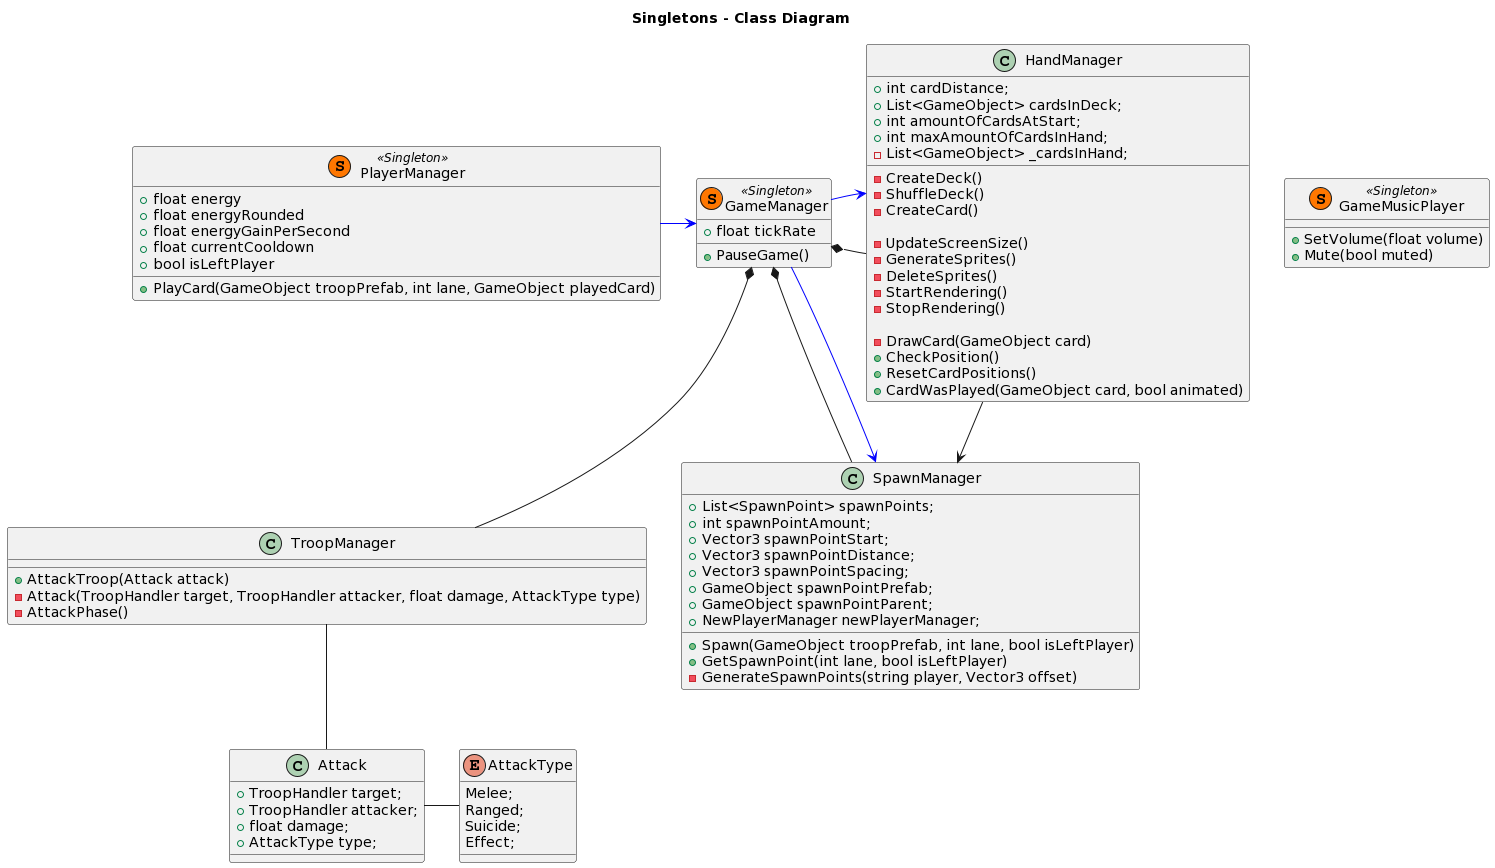
\includegraphics[width=13cm]{resources/Singletons.png} \\
    \caption{momentaner Aufbau}
\end{figure}

\begin{figure}[H]
    \centering
    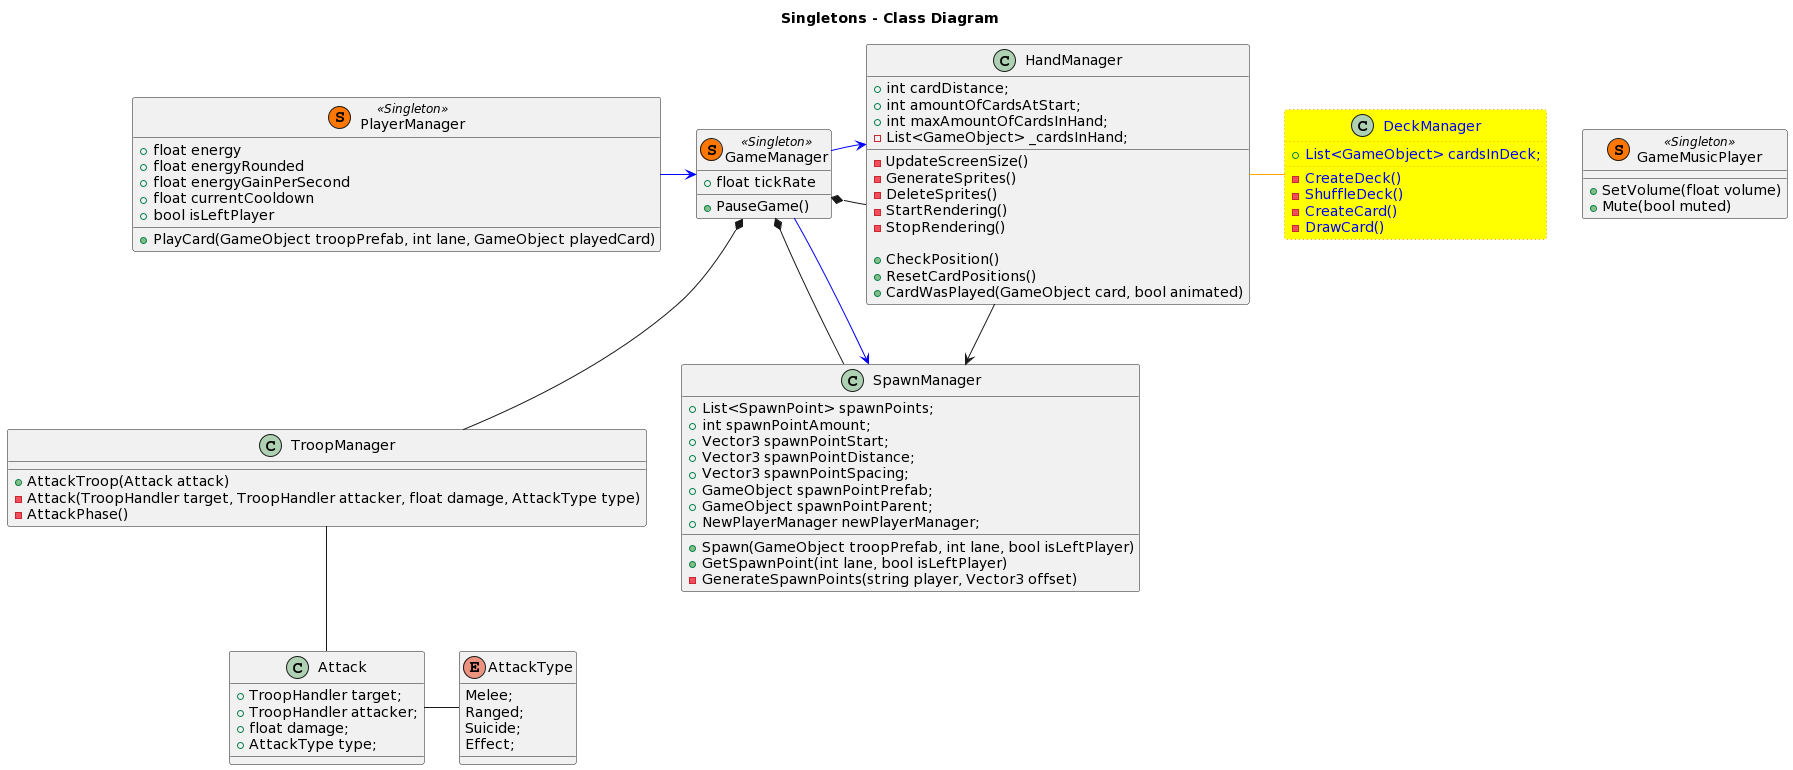
\includegraphics[width=13cm]{resources/Singletons 2.png} \\
    \caption{zukünftiger Aufbau}
\end{figure}

\section{Sequenzdiagramme}
\subsection{Nahkampftruppe}
\begin{figure}[H]
    \centering
    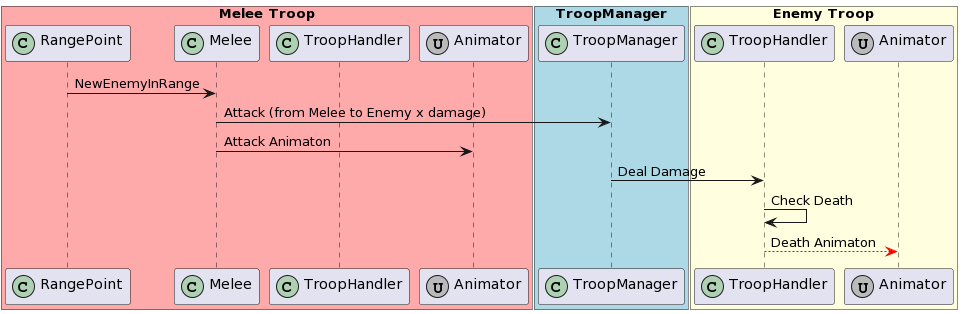
\includegraphics[width=15cm]{resources/MeleeAttacks.png}\\
    \caption{Abfolge, wenn eine Truppe in Reichweite einer Nahkampftruppe kommt}
\end{figure}

\subsection{Suizidtruppe}
\begin{figure}[H]
    \centering
    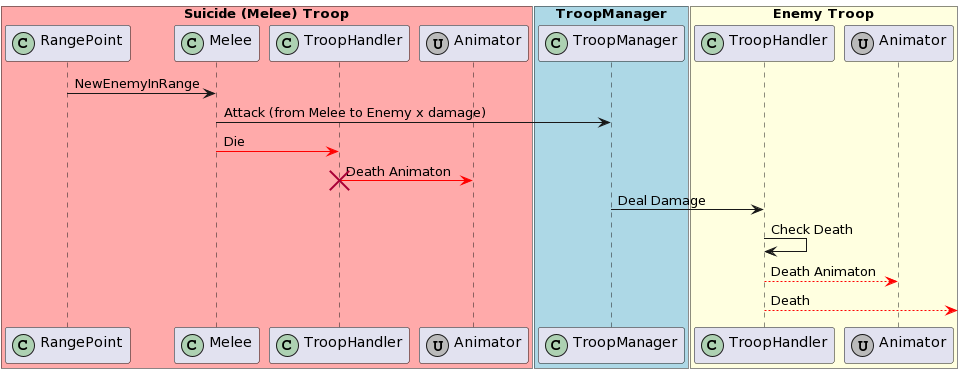
\includegraphics[width=15cm]{resources/SuicideAttacks.png}\\
    \caption{Suizidtruppe mit ähnlichen Prinzipien}
\end{figure}



\subsection{Fernkampftruppe}
\begin{figure}[H]
    \centering
    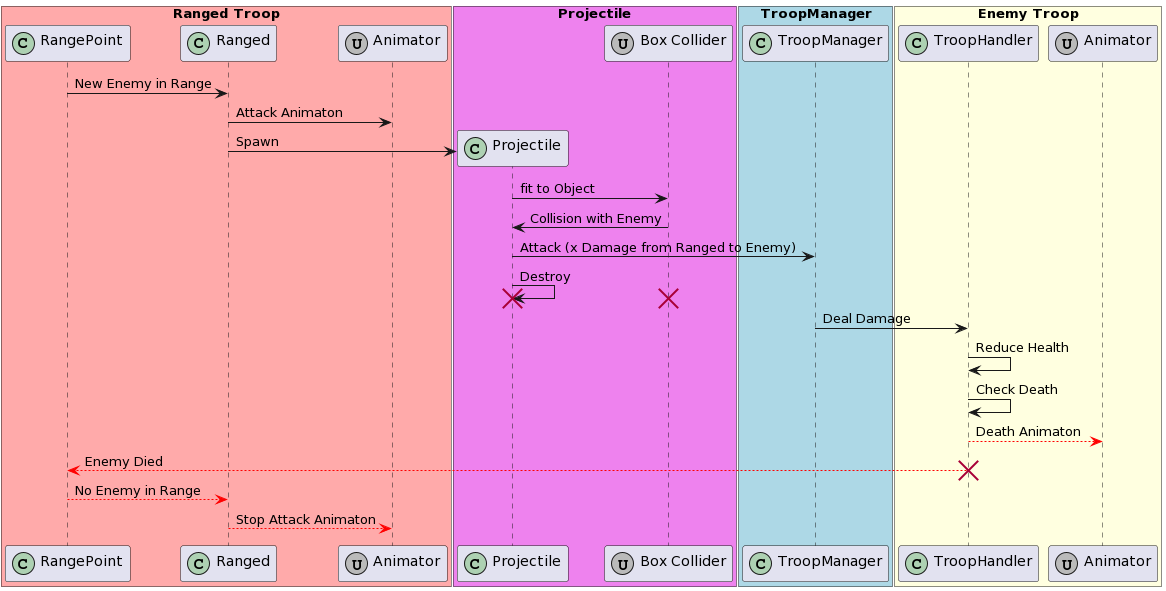
\includegraphics[width=15cm]{resources/RangedAttacks.png}\\
    \caption{Reaktion einer Fernkampftruppe auf neuen Gegner}
\end{figure}
\begin{figure}[H]
    \centering
    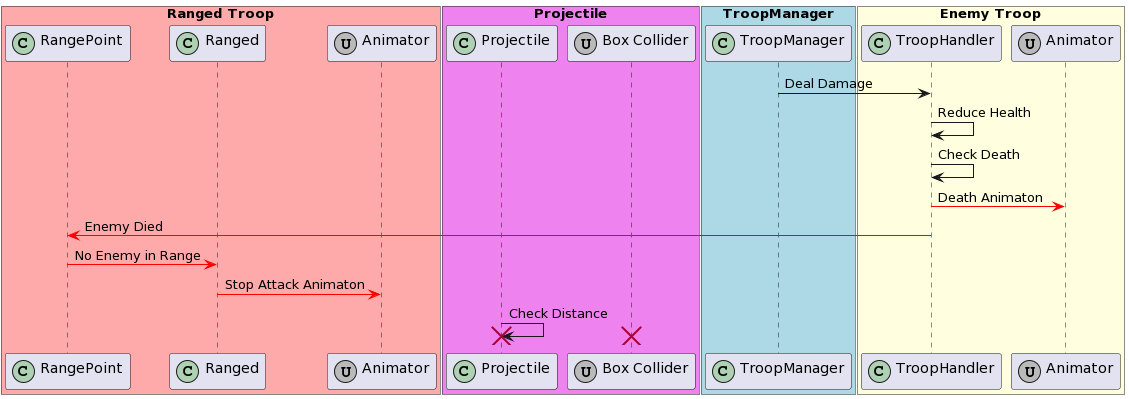
\includegraphics[width=15cm]{resources/Projectile.png}\\
    \caption{Gegner stirbt bevor das Projektil Schaden anrichten konnte}
\end{figure}


\subsection{Gift}
\begin{figure}[H]
    \centering
    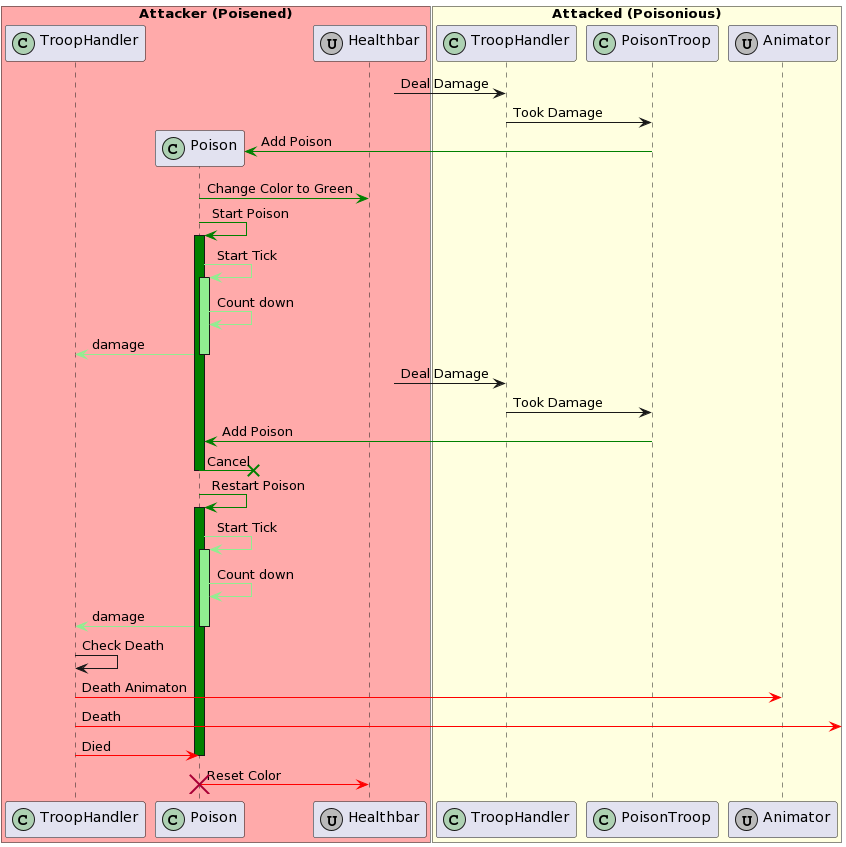
\includegraphics[width=15cm]{resources/Poison.png} \\
    \caption{Reaktion einer Truppe die den Effekt Gift besitzt}
\end{figure}


\section{GitHub source control}
Die Visualisierung von unserem GitHub Repository kann man unter folgendem \href{https://www.youtube.com/watch?v=IQT37uwpcg4}{Link} einsehen.
\input{02_produkt/03_Zukunft}

\part{Organisation}
\chapter{Technologien}

\section{\href{https://unity.com/}{Unity}}
''Unity ist mehr als eine Engine'', schreibt Unity auf der eigenen \href{https://unity.com/pages/more-than-an-engine}{Webseite}. Fakt ist, Unity ist die marktführende Game-Engine. Die Laufzeit- und Entwicklungsumgebung 
ist vor allem bei \gls{Indie Developer}n sehr beliebt. Deswegen ist es auch kein Wunder, dass über 50 Prozent aller Spiele mit Unity erstellt wurden. 
Doch auch für Grafikdesigner, Architekten, Filmentwickler und viele Weitere ist Unity ein sehr mächtiges Programm. Und wenn selbst die Streitkräfte der Vereinigten Staaten Unity nutzen, wieso sollten wir 
noch weiter suchen? Trotzdem haben wir einige für uns wichtige Vorteile herausgesucht:\\

\begin{itemize}
    \item Physik
    \begin{itemize}
        \item Unity berechnet einen grossen Teil der physikalischen Eigenschaften automatisch. Dies ist für uns von grossem Vorteil, da wir uns zum Glück nicht mit dem Berechnen von Kollisionen herumschlagen müssen.
        Ausserdem erlaubt uns Unity die Physik nach Bestreben zu ändern und ganz nach unserem Willen zu formen.
    \end{itemize}
    \item Grafiken
    \begin{itemize}
        \item Die Animation von Grafiken ist dank Unity ziemlich einfach. So kann man beispielsweise eine Bildersequenz in Unity laden, und Unity formt daraus automatisch eine Animation. Jedes Spielobjekt kann seinen
        eigenen Animator haben. In diesem kann man verschieden Zuständen des Spielobjekts verschiedene Animationen zuweisen. Greift die Truppe zum Beispiel an, wird von der normalen Animation zur Angriffsanimation
        gewechselt.
    \end{itemize}
    \item Programmierung
    \begin{itemize}
        \item In Unity kann man Spielobjekten selbst geschriebene Programme, sogenannte Scripts, hinzufügen. Diese werden mit C\# geschrieben. Dies war von Vorteil, da wir bereits Erfahrung mit C\# hatten. 
    \end{itemize}
\end{itemize}

\section{\href{https://github.com/}{GitHub}}
GitHub ist die grösste webbasierte open-source Plattform. Auf ihr kann man Source Code speichern und teilen. Ein grosser Vorteil von GitHub ist, dass man immer zu vergangenen Versionen zurückgelangen kann.
Hinzu kommt, dass man verschiedene Versionen des Source Codes in sogenannten Branches speichern und verändern kann. GitHub speichert ausserdem jede Änderung am Code, die durchgeführt wurde. So entsteht eine History, die jede Änderung nachverfolgen lässt. 
Ein sehr grosser Vorteil von GitHub ist, dass man im Team in Echtzeit am gleichen Code schreiben kann. Unser grösstes Pro-Argument: Backup-Backup-Backup!
Alles wird gespeichert, und es gibt keine Gründe, sich die Festplatte mit Backups vollzuschreiben. \\
Eine Visualisierung von unserem \gls{GitHub Repository} kann man unter folgendem \href{https://www.youtube.com/watch?v=IQT37uwpcg4}{Link} finden.


\section{\href{https://www.jetbrains.com/rider/}{Jetbrains Rider}}
''Rider ist eine unglaubliche .NET-IDE mit der Power von ReSharper'', schreibt Jetbrains auf der eigenen Webseite. Dies können wir nur bestätigen. Rider hat zudem die Unity API integriert. Dadurch hat Rider eine
spezialisierte Codeinspektion für Unity. Treten Errors im Unity Editor auf, kann Rider direkt den Ursprung des Fehlers anzeigen. Das Debugging ist dadurch um einiges leichter und müheloser. 
Rider warnt User ausserdem vor schlecht geschriebenen Funktionen, die einen Performance-kritischen Effekt auf das Spiel haben könnten. 


\section{\href{https://www.atlassian.com/software/jira}{Jira}}
Jira ist ein webbasiertes Programm für Projektmanagement und Zeiterfassung. Dies ermöglichte uns genau zu erfassen, wie viel Zeit wir an einem bestimmten Problem gearbeitet haben. Uns war klar, dass wir eine Art 
der Zeiterfassung brauchten, denn im Nachhinein ist dies ein Ding der Unmöglichkeit. Das Dashboard ist für berechtigte Personen unter diesem \href{https://maturarbeit--eli-marc.atlassian.net/}{Link} einzusehen.

\section{\href{https://www.latex-project.org/}{LaTeX}}
LaTeX verwendet das Textsatzsystem TeX. LaTeX ist eine Software, die sich von anderen Textprogrammen unterscheidet. Im Gegensatz zu den gewohnten WYSIWYG (''What You See is what you get'') Editoren (wie z.B. Word)
braucht man zur Benutzung von LaTeX einen separaten Editor. LaTeX vereinfacht den Umgang mit TeX durch einfachere Befehle. Der grösste Vorteil an TeX ist, dass man sehr genau einstellen kann, wie alles aussehen soll.


\section{\href{https://stability.ai/}{Stable Diffusion}}
Stable-Diffusion ist ein State-of-the-Art, Deep-Learning Text-zu-Bild Modell. Es wurde 2022 vom Start-up Stability AI veröffentlicht. Es wird für die Generation von detaillierten Bildern verwendet. Wir wollten seit
Beginn der Arbeit eine sehr neue Technologie verwenden. Dann als Stable Diffusion veröffentlicht wurde, war uns klar, dass wir diese Chance nicht verpassen dürfen. Hier ergab sich, dass wir Stable Diffusion verwendet haben, um einen individuellen
Hintergrund und ein individuelles Icon zu generieren. Wir nutzten Ideen, eine schlechte Skizze und viele Stunden an Testen und Verbessern, um den Hintergrund und das Icon nach unserem Geschmack zu generieren.

\section{\href{https://code.visualstudio.com/}{Visual Studio Code}}
Visual Studio Code ist ein kostenloser Editor von Microsoft. Ein grosser Vorteil von Visual Studio Code ist, dass man Erweiterungen hinzufügen kann. Die Erweiterung \href{https://marketplace.visualstudio.com/items?itemName=James-Yu.latex-workshop}{''LaTeX Workshop''}
hat dabei das spezifische Syntax-highlighting hinzugefügt. Ohne jene Erweiterung sich die Benutzung von LaTeX um einiges schwerer gewesen.

\section{\href{https://gource.io/}{Gource}}
Gource ist eine gratis open-source Software, die perfekt für die Visualisierung von GitHub Repositories geeignet ist. Wir haben Gource für die Erstellung eines Videos genutzt, das als \href{https://www.youtube.com/watch?v=IQT37uwpcg4}{Visualisierung unseres Dateisystems}
dient.


\chapter{Team Management}

\section{Anfänge}
\begin{itemize}
    \item Bereits Mitte Januar 2022 fragte Marc Elia an, ob sie nicht zusammen die Maturitätsarbeit schreiben wollten. Wir hatten beide vor, als Maturaarbeit etwas zu programmieren. Also vereinigten wir unsere Kräfte.
    \item Die nächste Frage war, was wir genau als Projekt programmieren wollten. Es stellte sich sehr schnell heraus, dass sich Marcs Grundidee (ein Videospiel) perfekt eignen würde. Man kann seiner Fantasie bei der Erstellung eines Videospiels
    freien Lauf lassen.
    \item Marc brachte am Anfang direkt den Vorschlag, dass wir unsere Zeit mit Jira tracken würden. Er setzte zudem GitHub und Unity für unseren ersten Gebrauch auf. 
    \item Elia konnte sich sehr schnell in dieser unbekannten Umgebung zurechtfinden. So entstand ein begeistertes, gleichberechtigtes Duo.
\end{itemize}

\section{Betreuungsperson}
\begin{itemize}
    \item Uns wurde vor Beginn der Arbeit mehrfach gesagt, dass einige Schüler*innen Probleme haben, eine Betreuungsperson zu finden. Um sicherzugehen, dass dies uns nicht geschehen würde, suchten wir bereits sehr früh nach einer Lehrperson.
    \item Elias erster Vorschlag war Herr Albert Kern. Er hat ihn bereits vor längerer Zeit provisorisch für eine individuelle Betreuung angefragt. Was lag näher, als ihn nun auch für eine Gruppenarbeit anzufragen? Wie es der Zufall wollte, begegneten sich 
    Herr Kern und Elia Ende Februar zufälligerweise auf dem Gang und tauschten einige Worte aus. Herr Kern gab allerdings zu, dass er keine Erfahrung mit der Entwicklung von Videospielen hatte und schlug Herrn Martin Hunziker vor.
    Dieser sei ein begnadeter Videospiel-Fanatiker und wahrscheinlich besser für die Betreuung geeignet. 
    \item Am dritten März schrieben wir per E-Mail eine kurze Anfrage an Herrn Hunziker. 
    Bereits vier Tage später sassen wir mit Herrn Hunziker in seinem Büro und besprachen mit ihm unsere Ideen. Er sagt uns, er habe selbst bisher keine Erfahrung in der Programmierung von Videospielen.
    \item Eine Woche später gab er sein schriftliches Einverständnis für die Betreuung unserer Maturitätsarbeit. 
    \item Wir informierten ihn regelmässig über unseren Fortschritt und konnten uns bei Fragen an ihn wenden.
\end{itemize}

\section{Kommunikation}
\begin{itemize}
    \item Die Kommunikation zwischen Elia und Marc fand vor allem über WhatsApp statt. Dies geschah allerdings nicht nur in Textform, sondern des Öfteren auch in Telefonaten zu allen möglichen, aber auch unmöglichen Uhrzeiten. Zudem konnten wir auf Jira nachschauen, auf welche Aufgabe der Partner
    seine Zeit getracked hat. 
    \item Zudem trafen wir uns dreimal physisch ausserhalb der Schulzeit, um unsere Arbeit zu organisieren.
    \item Wir müssen allerdings zugeben, dass die Kommunikation teilweise nicht ausreichend vorhanden war. Manchmal hatten wir keine Ahnung, woran genau der Partner arbeitete. Wir wussten zwar den ungefähren Arbeitsinhalt, allerdings nicht immer alle Einzelheiten.
    \item Die Kommunikation zwischen Schüler und Lehrer war unserer Meinung nach mit sechs Treffen genügend gut.
\end{itemize}




\chapter{Personal Reports}

\section{Team Review}
Generally, whenever we had a question, other members were happy to help and could provide helpful input.
The team was motivated to work on the project and work together to get everything done.
It was good that we invested extra time in the beginning, to set up a good architecture and have clean code, which made it very easy to create new features/endpoints.
There were times when it was a little challenging working in a team because of waiting dependencies, where one had to wait until someone finished something before you could continue working, which caused some delays.
Nevertheless, we managed very well, especially after noticing this issue and setting internal deadlines during the spring to prevent this, and it got much better.
After the large documentation block, we all wanted to start coding and focused less on creating informative Jira tickets.
Minimal task descriptions often lead to further questions or having to change something again.
Pascal-dependency was something we could improve on in the future, as he was often the person we contacted to answer questions, give more input on tasks and review our changes.
In the last weeks, we agreed on trying to reduce this dependency with the usage of public chats, asking questions as comments on issues instead of direct messages.
If we'd start the project from new again, we'd invest time into frontend testing, as nearly all our bugs were caused by the frontend, and we don't have any automated testing there.

\section{David}
Overall I'm happy with the whole project and enjoyed working on it.
I had the opportunity to learn new technologies (Kotlin, jOOQ, ktor, pinia) and improve my knowledge of already known ones (javascript, vue.js).
In a future project, I'd plan out my time better to prevent it all heaping up on the weekend and try to spread it out more under the week, which makes achieving the deadlines easier.
In the beginning, I had to ask for help regarding certain technologies, but it became less with time after working with them for a while.
In these past weeks, I feel like I've improved my skill set and can take my learnings with me to the next project.
My highlight was seeing everything coming together from the original idea and then being able to play a round of Jass after a few weeks.

\section{Pascal}
Overall, I really enjoyed our project and have no major complaints.
We chose a very adequate tech stack for our problem scope, and I wouldn't change any technology when starting over.
My personal highlight was the last three weeks when everybody got to work on new features, and we were able to extend our software without any significant roadblocks.
However, there is one thing I would do differently, the requirements engineering.
I tried my best to present reasonable requirements in my role as product owner, but that wasn't enough.
We should've prioritized the requirements from the beginning and spent more time questioning potential end-users to tailor our solution in a better way.

\section{Jamie}
With this project, I had the opportunity to get to know a lot of new technologies.
At the beginning of the project, I was hesitant to ask for help, which created some delays.
I learned that there is a balance of knowing when you should ask for help.
For future projects, I think I would invest more time in the requirement engineering and time management aspect of the project.

\section{Marcel}
I enjoyed working on the project, and I am happy with the end result.
I was able to deepen my knowledge of Kotlin, Vue.js and TypeScript and got to learn a cool framework with Ktor.
I could also bring my knowledge of SQL into the project and implemented all the database migrations.
In the middle of the project I did not always put enough time into the project, which meant not always meeting my sprint goals.
I was able to correct this for the last half of the project and was almost always able to get my tasks done within a sprint.
This project was also my first contact with the onion architecture style, as I was previously more familiar with layered architectures that are more tightly coupled to the database.


\part{Reflexion}
\chapter{Elia}

\section{Rückblick}
Das Produkt dieser Arbeit erfreut mich sehr. Obwohl dem Prototyp unseres Videospiels noch einige Funktionen fehlen, bin ich doch grundsätzlich mit unserem Spiel zufrieden. \\
Dies ist sehr wahrscheinlich das grösste und zeitaufwendigste Projekt, an dem ich jemals gearbeitet habe. Unser GitHub Repository enthält mehr als 40'000 Zeilen an C\# Source-Code.
Das ganze Repository ist ca. 1.1 Millionen Zeilen lang und mehrere Gigabytes gross (einschliesslich DLL's etc.). \\
Alleine hätte ich dies nie geschafft, deshalb bin ich besonders froh, dass wir dies im Team verwirklichen konnten. Die Gruppenarbeit hat mir viel Druck von den Schultern genommen, da ich mich bei Problemen immer auf Marc
verlassen konnte. Zudem führte die Zusammenarbeit zu vielen guten Ideen, die wir auch nur zusammen als Team in die Tat umsetzen konnten. Durch dieser Gruppenarbeit wurde  unsere Freundschaft stark gestärkt.
Ich habe zu schätzen gelernt, dass ich mich die ganze Zeit voll und ganz auf Marc verlassen konnte.\\
Obwohl von Anfang an klar war, dass dies eine sehr aufwendige Arbeit sein würde, habe ich sie doch unterschätzt. Am meisten unterschätzt habe ich allerdings den Arbeitsaufwand der schriftlichen Arbeit. Diese stellte sich als ziemlich grosser Zeitschlucker heraus. \\
Ich hatte zudem unterschätzt, was mein geplantes Hardwareupgrade für immensen Einfluss auf meinen Arbeitsfluss haben würde. Der Wechsel von meinem Laptop auf einen hochmodernen Computer brachte viele Vorteile mit sich.
Die vervielfachte Leistung hatte den Vorteil, dass ich bei Kompilierung des Codes keine halbe Minute mehr warten musste. Stattdessen konnte ich zwei Sekunden später unser Spiel testen.
Diese immense Rechenleistung merkte man auch daran, dass sich mein Zimmer durch die Nutzung des Computers im Laufe eines Tages trotz geöffnetem Fensters um mehrere Grade erwärmte.\\
Auch wenn die Fehlersuche teilweise sehr anstrengend war, hat mir das Programmieren, trotz teilweise langen Tagen und Nächten, meistens Spass gemacht. Ich fand es trotzdem Schade,
dass ich teilweise den ganzen Tag nur im Zimmer sass und an der Maturaarbeit programmierte. 

\section{Nächstes Mal}
Für das nächste Mal möchte ich mir zu Beginn des Semesters einen Plan erstellen, der festlegt, dass ich pro Woche mindestens eine Stunde arbeiten werde. Mit diesem Plan wäre es auf keinen Fall zu dieser sehr langen
Pause (von Mai bis August) gekommen. Wenn ich erneut die Chance hätte, dieses Projekt in einer Gruppenarbeit zu lösen, würde ich diese Chance ohne zu zögern ergreifen. Allerdings würde ich in Zukunft
unsere Organisation zwingend verbessern. Eventuell wäre ein drittes Teammitglied auch keine schlechte Idee (vgl. \autoref{chap:neusm}).\\
Was diese Erfahrung allerdings mit meinem Plan, Informatiker zu werden, geändert hat, kann ich zu diesem Zeitpunkt nicht beantworten. Fakt ist, ich habe nun auf jeden Fall eine genauere Vorstellung,
wie das Leben eines Informatikers aufgebaut ist. Zudem habe ich eine Menge an Respekt für jeden Spielentwickler gewonnen. Ein Spiel zu entwickeln ist nicht leicht, deswegen werde ich ab nun immer meine Erfahrungen im Hinterkopf
behalten, und auch immer an das Dev Team denken, wenn ich über einen Bug oder Crash fluche.
\chapter{Marc}

\section{Rückblick}
Im Grossen und Ganzem bin ich sehr zufrieden mit unserer Arbeit.
Allerdings war meine ursprüngliche Vorstellung unseres Spiels ausgereifter.
Dies scheiterte aber weder an Elia, mir oder uns beiden, sondern einfach an meiner Überschätzung.
Ich habe vor Jahren die selbe Spielidee auf eigene Faust versucht umzusetzen und kam in relativ wenig Zeit sehr weit.
Ich dachte der Fortschritt ist Linear.
Jedoch stiessen wir auch hier auf das Paretoprinzips: 20\% Aufwand gleich 80\% Ergebnis und die restlichen 20\% Ergebnis benötigen 80\% des Aufwands.
Der Feinschliff des UI-Aussehen, der Abschluss der schriftlichen Arbeit und ein bugfreies Spiel waren einige dieser massiv unterschätzten Zeitfresser. \\
Ich bin extrem froh Elia als Partner angefragt zu haben.
Ich habe mich gut mit ihm verstanden und denke er war für das Spiel mindestens gleich bereichernd wie ich.

\section{Nächstes Mal}
Ich denke eine minimal Anzahl Stunden die ich jede Woche erreichen möchte hätte geholfen.
Alleine eine Stunde hätte vermieden, dass ich jemals aus meinem Flow rausgelofen wäre.
Auch wäre aus dieser Stunde häufig mehr geworden. \\
Das überschätzen hatte nicht zu grafierende Folgen.
Es hat tatsächlich auch viel Motivation mit sich gebracht.
Jedoch hätten unnötige Zukunftsideen nicht sein müssen.
Dies haben wir bereits in der Team Reflexion unter "Verschwendete Zeit" genauer erklärt. \\
Entgegen der unerfüllten Erwartung bin ich stolz auf uns und denke wir haben für zwei Gymischüler ein brilliantes Produkt erstellt.
Nichtdestotrotz würde ich eine dritte Person mit ins Boot holen.

\chapter{Team}

\section{Rückblick}

\subsection*{Teamarbeit}
Wir verstanden uns während der ganzen Arbeit sehr gut. Es kam nie zu zwischenmenschlichen Problemen. Jedoch haben wir viel Potenzial der Teamarbeit nicht ausgeschöpft.
Teilweise war der Arbeitsprozess leider vergleichbar zu dem zweier Schüler, die am gleichen Projekt arbeiten. Dies hat zur Folge, dass es teilweise Code gibt,
den nur einer von uns richtig gut versteht. Diese ''Spezialitäten'' führten teils zu einem recht getrennten Arbeitsprozess. Zurückführen könnte man dies auch auf die zu seltenen
Treffen. Hätten wir uns öfter als dreimal getroffen, wären viele Unklarheiten oder Missverständnisse nicht aufgetreten. So waren wir beide des Öfteren unsicher, wie genau wir unsere verrichtete Arbeit
dokumentieren sollten. Es stellte sich zudem die Frage, was genau als investierte Zeit geltet.
Unser grösster Fehler war allerdings, dass wir keinen Schutzmechanismus für die Fehler einer Person eingeführt hatten. So war es für uns beide möglich, direkt am Hauptcode Änderungen vorzunehmen.
Hätten wir etwas dagegen vorgenommen, hätten wir keine 5 Stunden wegen eines kleinen Rechtschreibfehlers verloren.


\subsection*{Agilität}
Ein weiterer negativer Punkt unserer Projektplanung ist die entstandene Steifheit. Ein Ziel vor den Augen zu haben und eine Vision zu verfolgen ist wichtig. Jedoch soll es
immer möglich sein, diese anzupassen. Bereits im März haben wir sehr viel getüftelt und Ideen entwickelt, die zu diesem Zeitpunkt vollkommen irrelevant sein sollten.
So hatten wir beispielsweise bereits acht Effekte ''erfunden'', bevor es einen Prototyp gab.\\
Ohne es zu wissen, haben wir das Wasserfallmodell angewandt. Das Modell wird in der Informatik teils als eher schlecht erachtet, da man sich in der modernen
Entwicklung eher auf einen agilen Arbeitsprozess fokussieren sollte. Im Nachhinein müssen wir zugeben, dass wir fast allen möglichen Problemen des Wasserfallmodells
über den Weg gestolpert sind (\url{https://de.wikipedia.org/wiki/Wasserfallmodell#Probleme_und_Nachteile}).


\subsection*{Priorisierung}
Wir hatten im Allgemeinen eine teils ungenaue Priorisierung. Obwohl wir bereits ziemlich früh unsere Anforderungen festlegten, haben wir uns zum Teil in das eine oder andere verbissen.
Dies führte dazu, dass unter Umständen die Entwicklung von wichtigen Anforderungen für unwichtigere Funktionen pausiert wurde. 


\subsection*{Manpower} \label{chap:neusm}
Wir hatten gegenüber einer standardmässigen Maturitätsarbeit den Vorteil, dass wir zu zweit mehr Manpower mitbringen. Doch selbst unserem Duo sind zu zweit Grenzen gesetzt.
Aus diesem Grund sind wir uns einig, dass eine dritte Person beträchtlich bei der Arbeit geholfen hätte. Eine Möglichkeit wäre gewesen, dass das dritte Teammitglied die ganze
gestalterische Arbeit übernommen hätte. Doch auch ein weiterer Entwickler hätte massgebend bei der Arbeit ausgeholfen. Zudem denken wir, dass ein Team mit drei Mitgliedern
immer noch recht klein ist. Aus diesem Grund hätte ein dritter Arbeitspartner zu keinen grossen Team-Management-Problemen geführt.


\subsection*{Dokumentation}
Wir haben den Beginn der schriftlichen Arbeit zu spät angesetzt. Zu Beginn hatten wir eine sehr genaue, fast schon abgabebereite Dokumentation. Mit der Zeit ging dies allerdings verloren.
Gegen Ende stand nun in der Zeitnotierung lediglich die Funktion, die nicht funktioniert hatte, und nicht wie zu Beginn eine genauere Dokumentation die darlegt; was wo wieso genau nicht funktioniert hat.

\section{Nächstes Mal}

\subsection*{Treffen}
Eine höhere Anzahl an Treffen und Telefonaten würden eine höhere Klarheit bedeuten. Gäbe es eine weitere Arbeit, würden wir uns mindestens monatlich treffen, um den Stand der Dinge zu besprechen.\\
Mögliche Fragen, die auf diesem Weg einfacher zu klären sind, sind:
\begin{itemize}
    \item[-] ''An welchem Punkt stehen wir genau?''
    \item[-] ''Was haben die einzelnen Teammitglieder in der nächsten Zeit vor?''
    \item[-] ''Gibt es neue wichtige Ideen für das Spiel?''
    \item[-] ''Sind unsere alten Skizzen noch wahrheitsgetreu?''
    \item[-] ''Benötigen wir neue Skizzen?''
    \item[-] ''Was sind die nächsten Schritte?''
\end{itemize}


\subsection*{Vier-Augen-Prinzip}
Üblich bei der Nutzung von GitHub als Team sind sogenannte Pull-Requests. Diese finden statt, wenn ein Mitglied eine Änderung auf den Hauptordner übertragen will. Ein solcher
Pull-Request muss dann von einem weiteren Teammitglied genehmigt werden. Der Hintergrundgedanke ist, dass das zweite Mitglied den Code ebenfalls auf mögliche Fehler untersucht.
Dieser Weg reduziert die Anzahl an Fehlern und erhöht somit auch die schlussendlich gesparte Zeit. In einer weiteren Arbeit würden wir dieses Prinzip ohne Ausnahmen anwenden.


\subsection*{Priorisierung}
Diesen Punkt anzupassen und anzuwenden ist eher schwierig. Mit einer grösseren Menge an Treffen, Besprechungen und Planung könnte man dieses Problem allerdings in der Zukunft
minimieren.


\subsection*{Verschwendete Zeit}
Die gesamte ''verschwendete Zeit'' beträgt lediglich wenige Stunden. Trotzdem haben wir zu Beginn den Fehler getätigt und zu weit in die Zukunft geplant. Ein Zeitverlust durch Fehler
sehen wir nicht als ''verschwendet'', sondern eher als ''Zeit des Lernens''. Durch das Beheben unserer Fehler haben wir sehr wahrscheinlich am meisten gelernt.
Es würde allerdings mehr Sinn ergeben, sich zu Beginn zu entscheiden, dass Effekte existieren werden. Zudem könnte man sich eventuell bereits ein Proof of Concept ausdenken.
Kommt man in der Entwicklung in ein Stadium, in dem die Zeit es erlaubt, kann man immer noch mehrere Ideen für Effekte erarbeiten. \\
Wir haben allerdings den Fehler gemacht, dass wir uns zu Beginn acht verschiedene Effekte erarbeitet haben. Dies hat uns wertvolle Planungszeit gekostet, die wir an anderen Stellen besser hätten nutzen können.


% Note: The project proposal needs to be included in the following way (i.e. using `\input` and not `\include`, and with the `\chapter` declaration outside the input{}-tag), since the proposal can also be generated as a stand-alone document.
% \chapter{Initial Project Proposal}
% \paragraph{Project name:} JassTracker

\subsubsection*{Team Members}

\begin{compactenum}
    \item Pascal Honegger (\href{mailto:pascal.honegger1@ost.ch}{pascal.honegger1@ost.ch})
    \item Marcel Joss (\href{mailto:marcel.joss@ost.ch}{marcel.joss@ost.ch})
    \item David Kalchofner (\href{mailto:david.kalchofner@ost.ch}{david.kalchofner@ost.ch})
    \item Jamie Maier (\href{mailto:jamie.maier@ost.ch}{jamie.maier@ost.ch})
\end{compactenum}

\subsubsection*{Availabilities}

% Table generated using https://www.tablesgenerator.com

\begin{flushleft}
    \begin{tabular}{|c|c|c|c|c|c|c|}
        \hline
        Time slot   & Mon  & Tue  & Wed  & Thu & Fri   & Sat \\ \hline
        08h00-09h00 & (XO) &  -   &  -   &  -  & (XO)  &  -  \\ \hline
        09h00-10h00 & (XO) &  -   &  -   &  -  & (XO)  & XO  \\ \hline
        10h00-11h00 & (XO) &  -   &  -   &  -  & (XO)  & XO  \\ \hline
        11h00-12h00 & (XO) &  -   &  -   &  -  & (XO)  & XO  \\ \hline
        \rowcolor[HTML]{EFEFEF}
        12h00-13h00 & (XO) & (XR) & (XR) & (XO) & (XO) & XO  \\ \hline
        13h00-14h00 & (XO) & XR   &  -   & (XO) & (XO) & XO  \\ \hline
        14h00-15h00 & (XO) & XR   &  -   & (XO) & (XO) & XO  \\ \hline
        15h00-16h00 & (XO) &  -   &  -   & (XO) & (XO) & XO  \\ \hline
        16h00-17h00 & (XO) &  -   &  -   & (XO) & (XO) & XO  \\ \hline
        \rowcolor[HTML]{EFEFEF}
        17h00-18h00 &  -   &  -   &  -   & (XO)  & (XO) &  -  \\ \hline
        \rowcolor[HTML]{EFEFEF}
        18h00-19h00 &  -   &  -   &  -   & (XO) & (XO) &  -  \\ \hline
    \end{tabular}

\end{flushleft}

\subsubsection*{Project Idea}

JassTracker is a web app which allows tracking and analysis of the popular Swiss card game ``\href{https://de.wikipedia.org/wiki/Jass}{Jass}''.
There are many forms of playing, but the one we're focusing on is called ``Coiffeur''.
The two teams have two players each and need to keep track of what they've already played and which options are available to them.
They also track whose turn it is, apply the correct multiplication to the score and sum it all up in the end.
To work around this, a project team member is currently using a excel spreadsheet, but this solution provides limited functionality and has many drawbacks.

To make the scoring easier JassTracker allows players to easily track, analyze and sync games digitally.
In a first step you will be able to create and arrange team members for a given game.
Then you start playing the game physically and assign scored rounds to the correct member.
During this phase you'll also be able to see live stats such as average score by player so far.
After the game some highlights (e.g.\ the best player) are highlighted.
You can also gain exhaustive insight into your play style by looking at personal or group statistics such as average score by player or historic averages.
To enable this, other physical members are able to associate their game to their personal account to track personal statistics across games.


Some potential ideas to expand on: configurable Jass game (e.g. Coiffeur with 8 instead of 10 options), prediction of scores based on past performance, current game trajectory (win probability by team).

\subsubsection*{Proposed Realization}

We plan on implementing a web app using \href{https://vuejs.org/}{Vue.js} as a frontend library.
For styling we plan on using \href{https://getbootstrap.com/}{Bootstrap} for basic styles.
The server will be implemented in Kotlin using the \href{https://ktor.io/}{Ktor} framework.
Persistent data is stored in a \href{https://www.postgresql.org/}{PostgreSQL} database and accessed using \href{https://www.jooq.org/}{jOOQ}.
Development will be done locally in \href{https://www.jetbrains.com/idea/}{IntelliJ IDEA}, production deployments will be using Docker containers.
CI / CD will be implemented using the OST GitLab.


% Ensure all entries are printed, even if not referenced
\glsaddall
\part{Glossar}
\printglossary
\newpage

\addcontentsline{toc}{chapter}{Bibliography}

% Ensure all citations are printed, even if not referenced
\nocite{*}

\bibliographystyle{alpha}
\bibliography{bibliography}

\end{document}
